%*****************************************
\chapter{Ausführung der Lösung und Ergebnisse}\label{ch:solution}
%*****************************************
In diesem Kapitel werden nun die im Kapitel \ref{ch:approach} vorgestellte Prozessschritte durchgegangen.
Nach jedem Prozessschritt werden die daraus resultierenden Ergebnisse präsentiert.

\section{Analyse}

Im ersten Schritt wird eine Analyse durchgeführt.
Hier werden zwei Techniken des User-Centered Designs angewendet.
Die Ergebnisse der Analyse sind Anforderungen an das Konzept der neuen Anwendung und drei Personas, die stellvertretend für die drei Zielgruppen im gesamten Entwicklungsprozess stehen.

\subsection{Befragung}

Die Befragung fand im Rahmen einer offenen Diskussion statt.
Bei der Diskussion waren Prof. Dr. Alfred Winter und Dr. Franziska Jahn beteiligt.
Als Leitweg der Diskussion wurde die Umfrage im Anhang \ref{analyse_umfrage} verwendet.
Die Umfrage bestand sowohl aus geschlossenen Fragen, wo die Befragten die aktuelle Lösung bewertet haben als auch aus offene Fragen, die zu einer Diskussion eingeladen haben.
So wurden Anforderung an die neue Anwendung gesammelt. \\

Die folgenden sechs Herausforderungen haben sich aus der Befragung abgeleitet:

\begin{enumerate}
\item \textbf{Intuitive Nutzerführung} \newline
Die Nutzerführung soll so konzipiert werden, dass Nutzer ohne großen Zeitaufwand und ohne langes Überlegen zum gewünschten Ziel kommen. 
Es sollen Navigationselemente (z.B. Menüs, Buttons) verwendet werden, die Nutzer*innen aus andere Anwendungen kennen und mit denen diese vertraut sind.
\item \textbf{Flexible Suche} \newline
Die Suche soll in einer Form gestaltet werden, dass jede Art von Suchanfragen gemacht werden können.
\item \textbf{\"Ubersichtliche Ergebnisseite} \newline
Die Ergebnisse der Suche sollen übersichtlich dargestellt werden.
Es sollen keine überschüssige Informationen angezeigt werden.
\item \textbf{\"Ubersichtliche Detailseite} \newline
Die Detailseiten von Softwareprodukte oder Studien sollen den Absprung ins RickView nicht mehr erlauben.
Die auf den Detailseiten dargestellten Informationen sollen von Menschen lesbar sein können.
\item \textbf{\"Ubersichtliche Darstellung der Kataloge} \newline
Die Struktur der Website soll um eine weitere Seite erweitert werden und zwar der Darstellung der Kataloge.
Da sollen alle Kataloge aus den unterschiedlichen Quellen angezeigt werden.
\item \textbf{Darstellung des Metamodells} \newline
Das Metamodell der Ontologie soll in die Benutzeroberfläche integriert werden, um die Herkunft der Daten nachvollziehen zu können.
\end{enumerate}

\subsection{Personas}

Personas sind die zweite Technik, die im Rahmen der Analyse ausgewählt wurde.
Die Persona-Typen haben sich durch die Motivation der Arbeit herauskristallisiert.
Es gibt insgesamt drei Zielgruppen und demnach sind die folgenden drei Personas entstanden:

\begin{itemize}
\item der/die \ac{CIO}
\item der/die Mitarbeiter*in im Krankenhaus
\item der/die Student*in
\end{itemize}

Im Folgenden werden die drei Personas ausführlich präsentiert.

\paragraph{Der/Die CIO} 

Lorem ipsum dolor sit amet, consetetur sadipscing elitr, sed diam nonumy eirmod tempor invidunt ut labore et dolore magna aliquyam erat, sed diam voluptua. 
At vero eos et accusam et justo duo dolores et ea rebum. 
Stet clita kasd gubergren, no sea takimata sanctus est Lorem ipsum dolor sit amet.

\begin{figure}[H]
	\centering
    	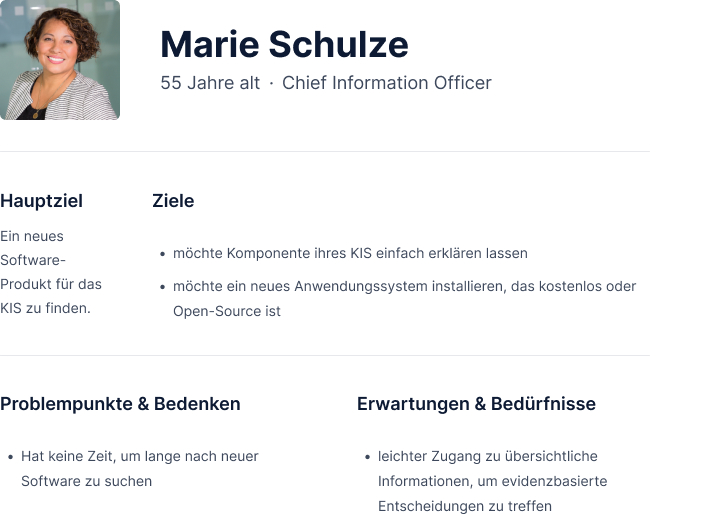
\includegraphics[width=1.1\textwidth]{Images/Persona_1}
   	\caption{Persona 1: CIO}
   	\label{fig:persona1}
\end{figure}

\paragraph{Der/Die Mitarbeiter*in im Krankenhaus}

Lorem ipsum dolor sit amet, consetetur sadipscing elitr, sed diam nonumy eirmod tempor invidunt ut labore et dolore magna aliquyam erat, sed diam voluptua. 
At vero eos et accusam et justo duo dolores et ea rebum. 
Stet clita kasd gubergren, no sea takimata sanctus est Lorem ipsum dolor sit amet.

\begin{figure}[H]
	\centering
    	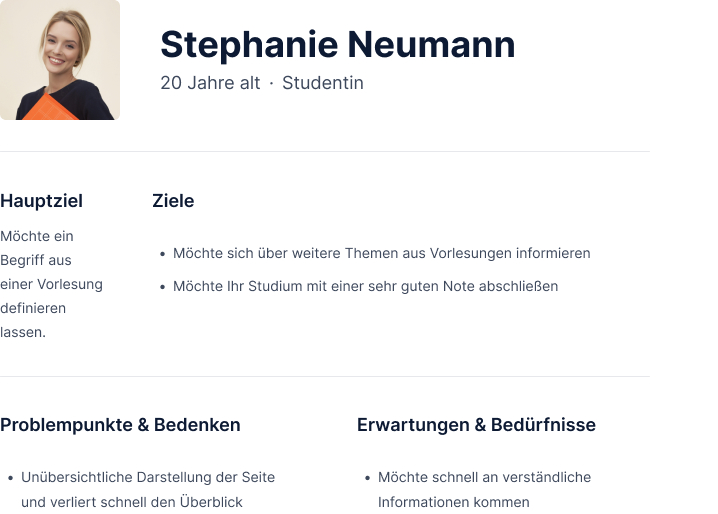
\includegraphics[width=1.1\textwidth]{Images/Persona_3}
   	\caption{Persona 2: Der/Die Mitarbeiter*in im Krankenhaus}
   	\label{fig:persona2}
\end{figure}

\paragraph{Der/Die Student*in} 

Lorem ipsum dolor sit amet, consetetur sadipscing elitr, sed diam nonumy eirmod tempor invidunt ut labore et dolore magna aliquyam erat, sed diam voluptua. 
At vero eos et accusam et justo duo dolores et ea rebum. 
Stet clita kasd gubergren, no sea takimata sanctus est Lorem ipsum dolor sit amet.

\begin{figure}[H]
	\centering
    	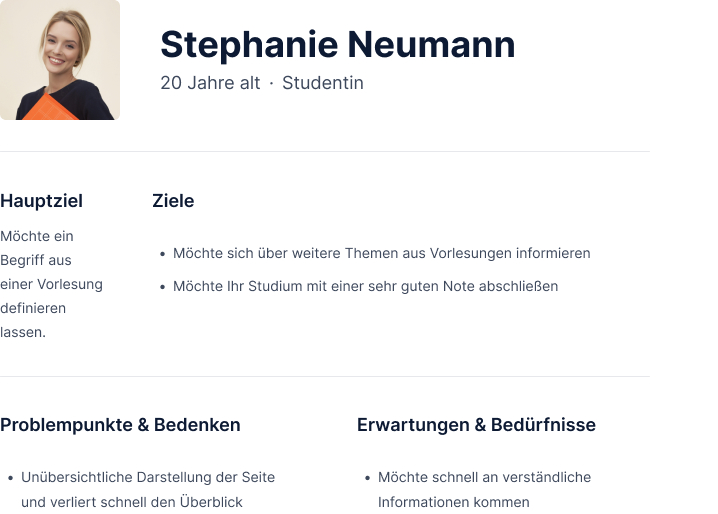
\includegraphics[width=1.1\textwidth]{Images/Persona_3}
   	\caption{Persona 3: Der/Die Student*in}
   	\label{fig:persona3}
\end{figure}

\section{Konzeption}

Im zweiten Schritt des nutzerzentrierten Entwicklungsprozesses können nun mit Hilfe der in der Analyse gewonnen Informationen die Wireframes erstellt werden.
Hierbei wurde jeweils ein Wireframe für die folgenden Seitentypen angelegt:

\begin{itemize}
\item Startseite
\item Ergebnisseite
\item Detailseite Softwareprodukt
\item Katalogübersicht
\end{itemize}

In diesem Schritt wurden zwei Iterationen durchgeführt.
Die erzeugten Wireframes aus der ersten Iteration, können im Anhang \ref{app_wireframes} gesichtet werden.
Nach der ersten Iteration, fand eine Zwischenevaluation statt.
Diese Zwischenevaluation wurde im Rahmen einer offenen Diskussion durchgeführt.
Gemeinsam mit Prof. Dr. Alfred Winter, Dr. Franziska Jahn und Dr. Konrad Höffner wurden die aus der ersten Iteration entstandenen Wireframes bewertet.
Das gesammelte Feedback wurde dann in der zweiten Iteration umgesetzt.
Im Folgenden werden die finalen Wireframes präsentiert.

\paragraph{Startseite}

Lorem ipsum dolor sit amet, consetetur sadipscing elitr, sed diam nonumy eirmod tempor invidunt ut labore et dolore magna aliquyam erat, sed diam voluptua. 
At vero eos et accusam et justo duo dolores et ea rebum. 
Stet clita kasd gubergren, no sea takimata sanctus est Lorem ipsum dolor sit amet.

\begin{figure}[H]
	\centering
    	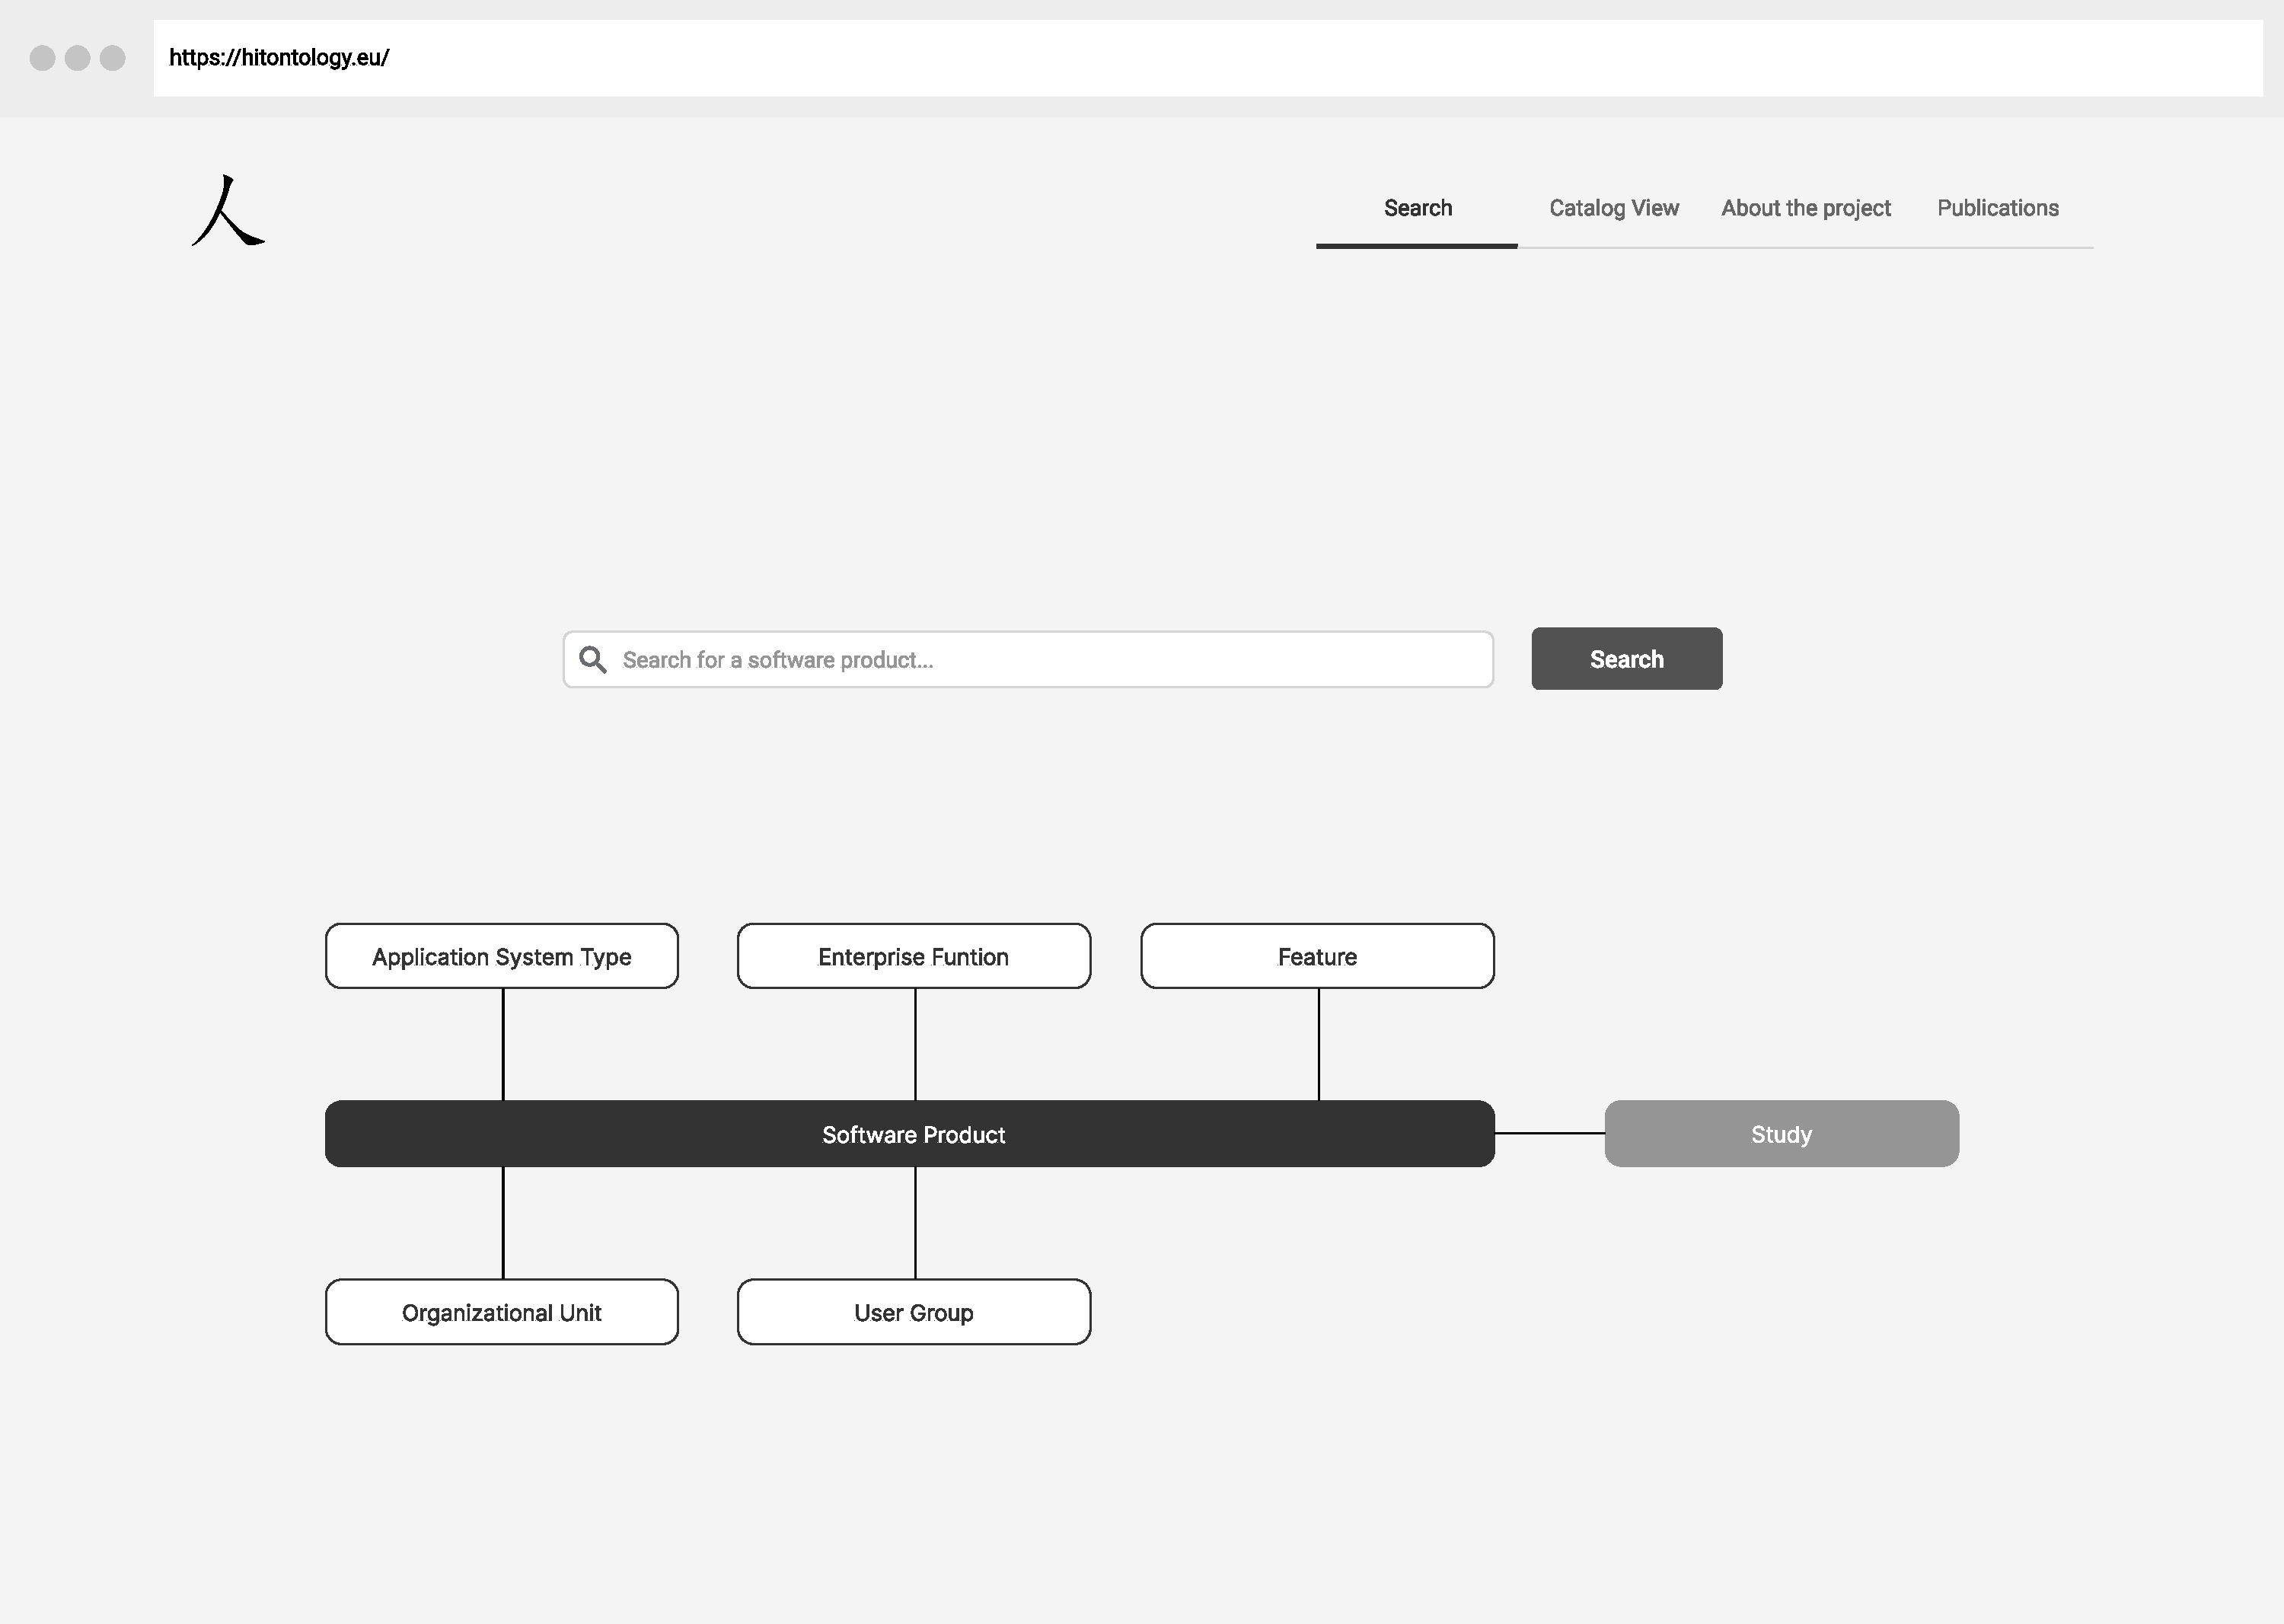
\includegraphics[width=\textwidth]{Images/Wireframe_Startseite}
   	\caption{Wireframe - Startseite}
   	\label{fig:wireframe_start}
\end{figure}

\paragraph{Ergebnisseite}

Lorem ipsum dolor sit amet, consetetur sadipscing elitr, sed diam nonumy eirmod tempor invidunt ut labore et dolore magna aliquyam erat, sed diam voluptua. 
At vero eos et accusam et justo duo dolores et ea rebum. 
Stet clita kasd gubergren, no sea takimata sanctus est Lorem ipsum dolor sit amet.

\begin{figure}[H]
	\centering
    	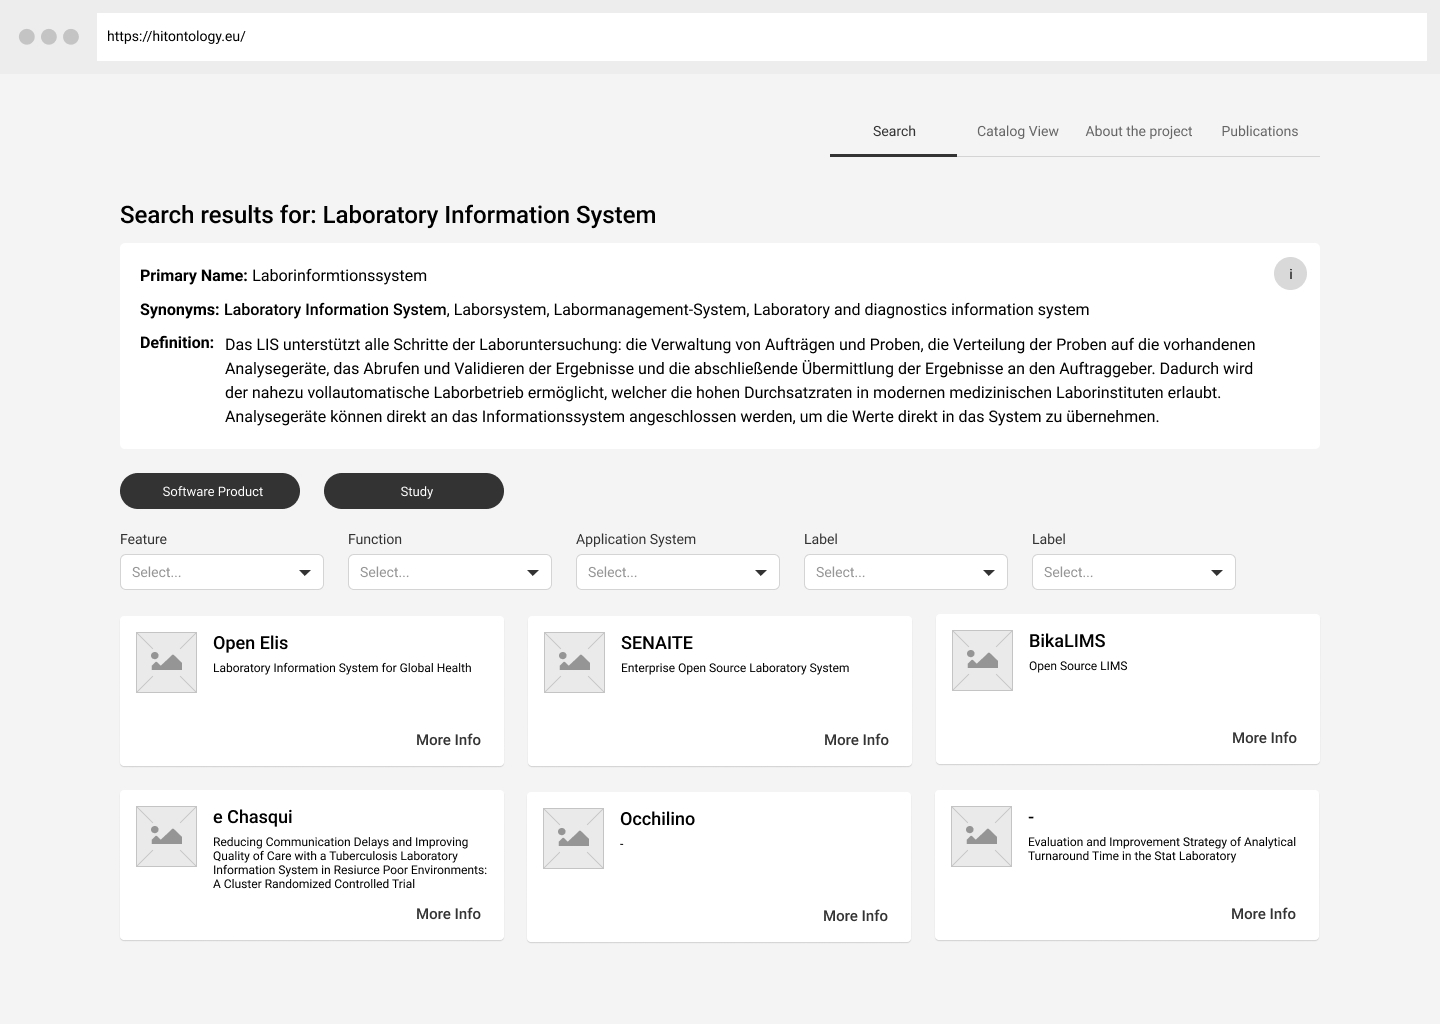
\includegraphics[width=\textwidth]{Images/Wireframe_Ergebnisseite}
   	\caption{Wireframe - Ergebnisseite}
   	\label{fig:wireframe_results}
\end{figure}

\paragraph{Detailseite Softwareprodukt}

Lorem ipsum dolor sit amet, consetetur sadipscing elitr, sed diam nonumy eirmod tempor invidunt ut labore et dolore magna aliquyam erat, sed diam voluptua. 
At vero eos et accusam et justo duo dolores et ea rebum. 
Stet clita kasd gubergren, no sea takimata sanctus est Lorem ipsum dolor sit amet.

\begin{figure}[H]
	\centering
    	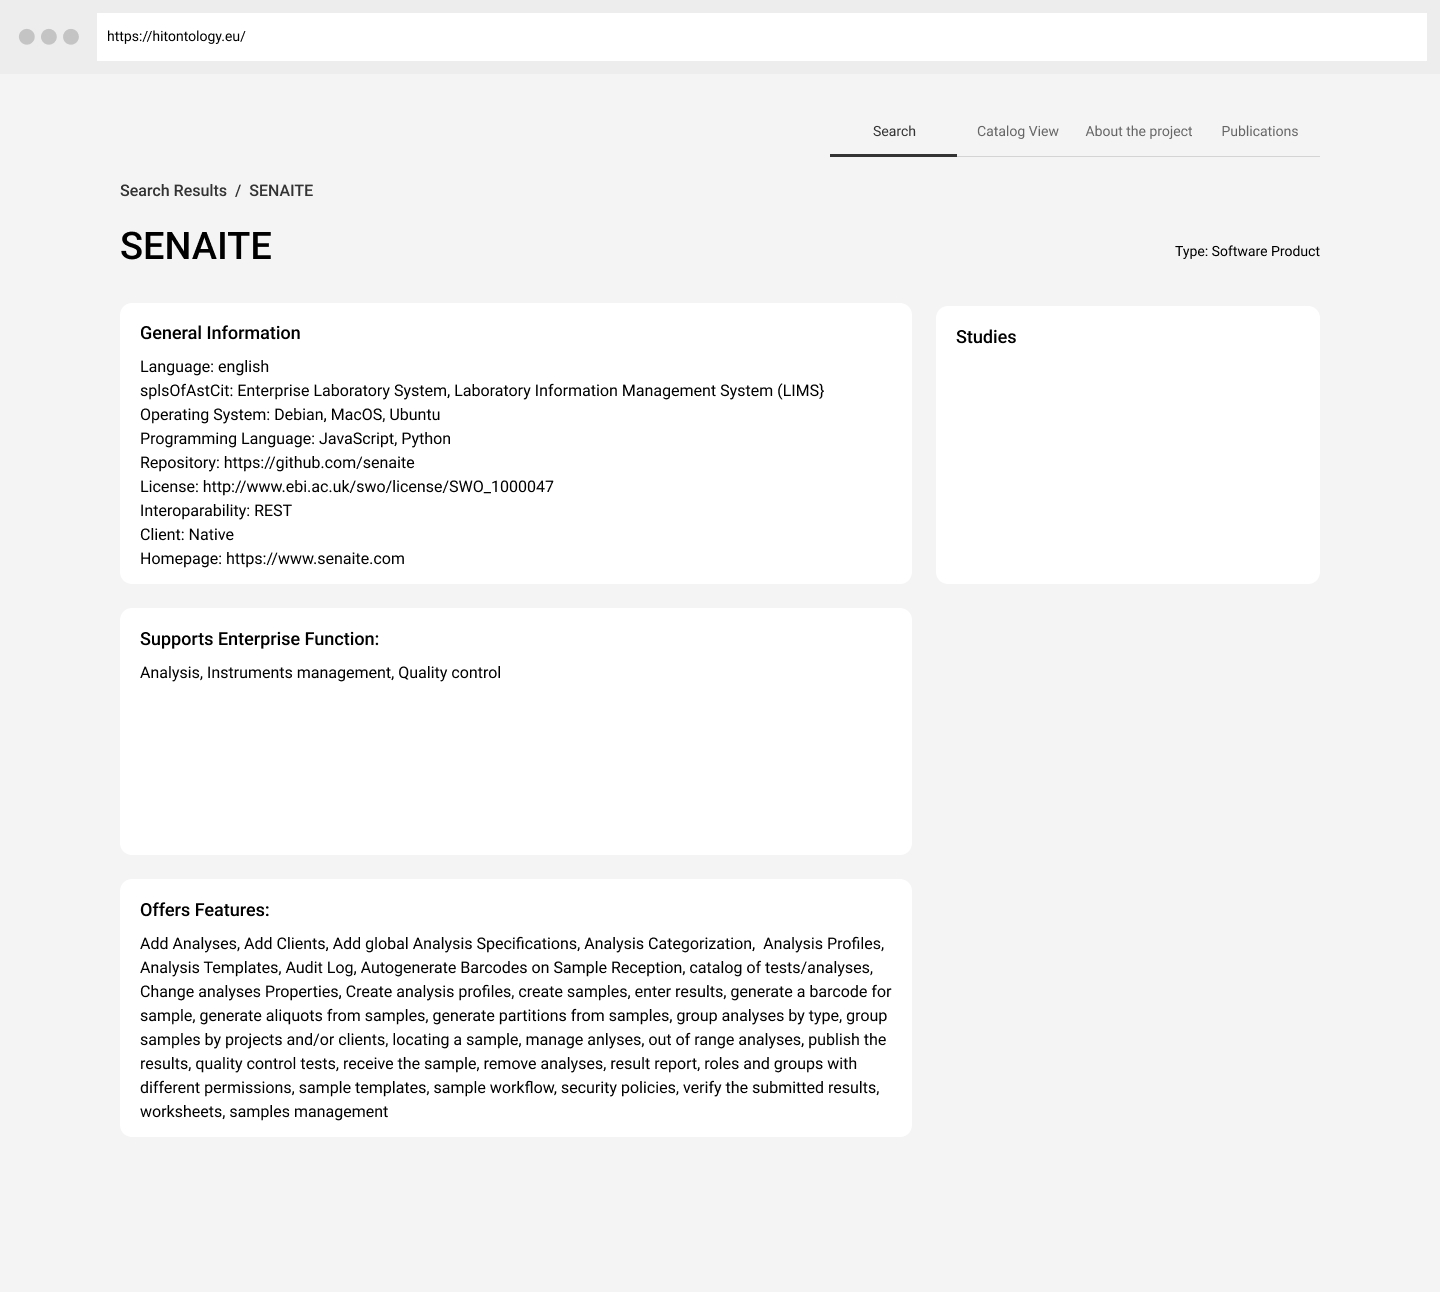
\includegraphics[width=\textwidth]{Images/Detail_SP}
   	\caption{Wireframe - Detailseite Softwareprodukt}
   	\label{fig:wireframe_detail_sp}
\end{figure}

\paragraph{Katalogübersicht}

Lorem ipsum dolor sit amet, consetetur sadipscing elitr, sed diam nonumy eirmod tempor invidunt ut labore et dolore magna aliquyam erat, sed diam voluptua. 
At vero eos et accusam et justo duo dolores et ea rebum. 
Stet clita kasd gubergren, no sea takimata sanctus est Lorem ipsum dolor sit amet.

\begin{figure}[H]
	\centering
    	\includegraphics[width=\textwidth]{Images/Wireframe_Katalogübersicht}
   	\caption{Wireframe - Katalogübersicht}
   	\label{fig:wireframe_catalogue}
\end{figure}

\section{Design}

Das Design der neuen Website lehnt sich an das Corporate Design von IMISE an.
Die ausgewählte Farbpalette ist in der Abbildung dargestellt.
Das 

\subsection{Mockups}

Im folgenden werden die finalen Screens der Anwendung erläutert.

\paragraph{Startseite}

Die Abbildung \ref{fig:mockup_start1} zeigt die Startseite der Website mit der inaktiven Wortsuche und einer vereinfachten Version des Metamodells der Ontologie.
Des Weiteren besteht auch die Möglichkeit, zwischen den unterschiedlichen Unterseiten der Website über das horizontale Menü zu navigieren.
Sobald Nutzer*innen ein Begriff in das Suchfeld eingeben, wird im Metamodell das zum Begriff zutreffende Katalog hervorgehoben.
Somit erhalten Nutzer*innen einen Einblick in der Herkunft der Daten.
Dieses Verhalten kann in der Abbildung \ref{fig:mockup_start2} beobachtet werden.

\begin{figure}[H]
	\centering
    	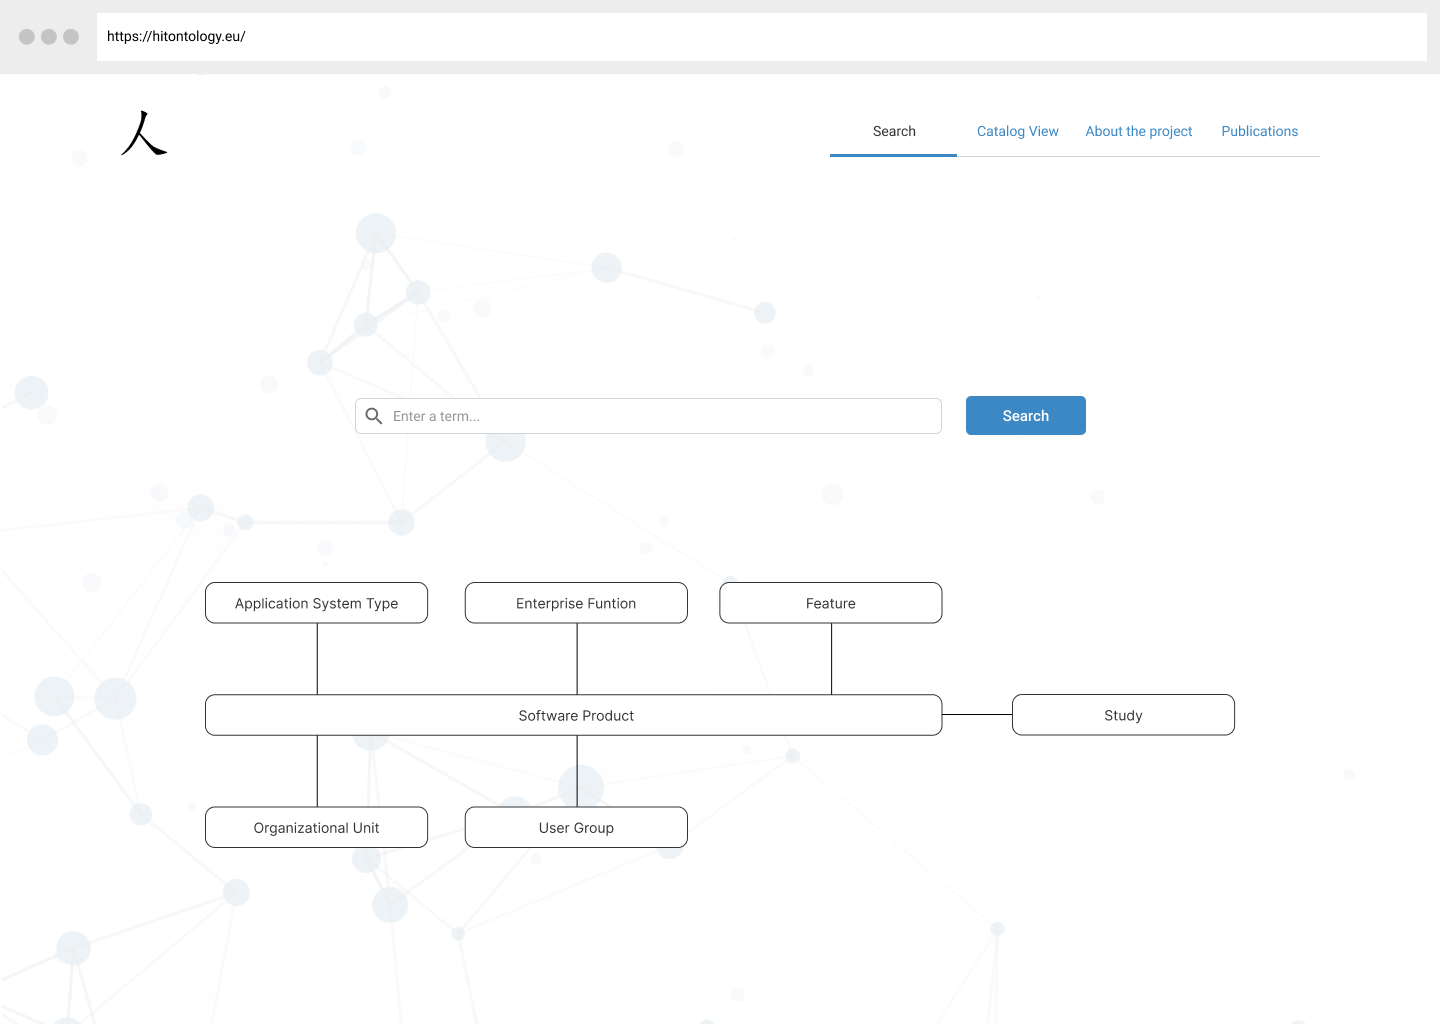
\includegraphics[width=\textwidth]{Images/Mockup_Startseite_1}
   	\caption{Mockup - Startseite}
   	\label{fig:mockup_start1}
\end{figure}

\begin{figure}[H]
	\centering
    	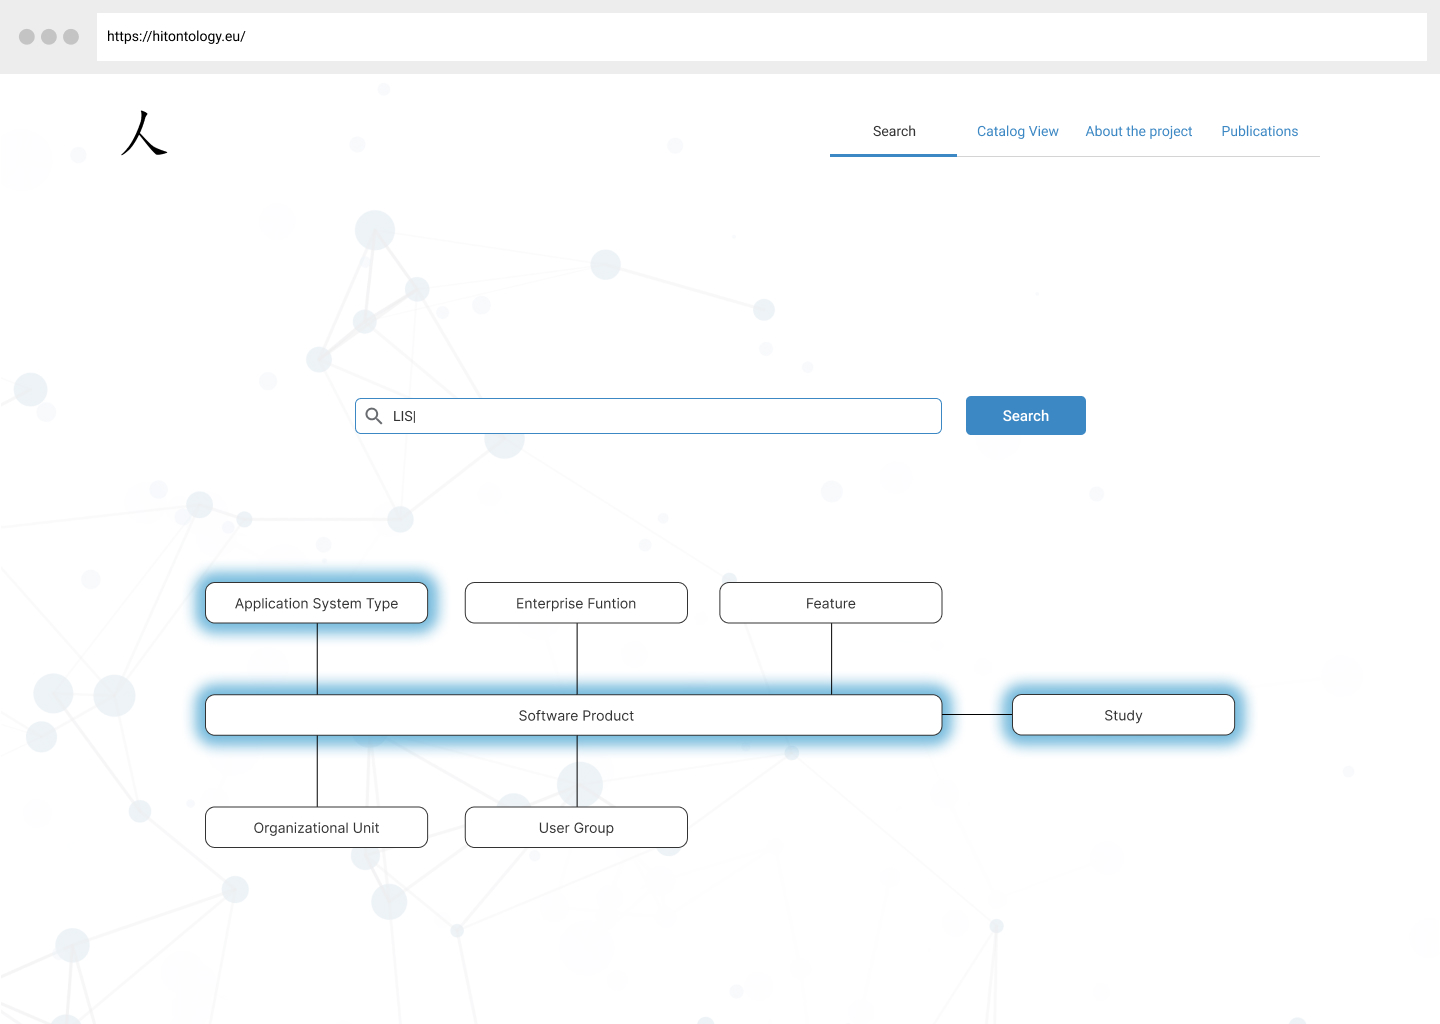
\includegraphics[width=\textwidth]{Images/Mockup_Startseite_2}
   	\caption{Mockup - Startseite mit aktiver Suche}
   	\label{fig:mockup_start2}
\end{figure}

\paragraph{Ergebnisseite}

Die Ergebnisseite enthält die folgenden Elemente:

\begin{itemize}
\item \textbf{Erklärung zum Suchbegriff} - hier werden Katalogbasiert Primärbezeichner, Synonyme Begriffe und eine Definition angezeigt. Nutzer*innen können hier dann auch zwischen unterschiedliche Kataloge auswählen und sich die darin existierenden Informationen anzeigen lassen.
\item \textbf {Filter} - Hier haben Nutzer*innen die Möglichkeit die Ergbenisse ihrer Suche zu verfeinern. Es steht Nutzer*innen zur Auswahl ob sie sich nur Softwareprodukte, nur Studien oder beides in der Ergebnisliste anzeigen lassen möchten. Des Weiteren können Sie die Ergebnisse anhand weiteren Filter anpassen wie zum Beispiel (hier noch mit Beispiele ergänzen).
\item \textbf{Ergebnisse} - Hier werden die zutreffenden Softwareprodukte und Studien zu dem Suchbegriff angezeigt. Softwareprodukte lassen sich mit Hilfe des dargestellten Icons auf der Kachel unterscheiden.
\end{itemize}

Die Abbildung \ref{fig:mockup_results} stellt beispielhaft die Ergebnisseite zu dem Suchbegriff \enquote{LIS} dar.

\begin{figure}[H]
	\centering
    	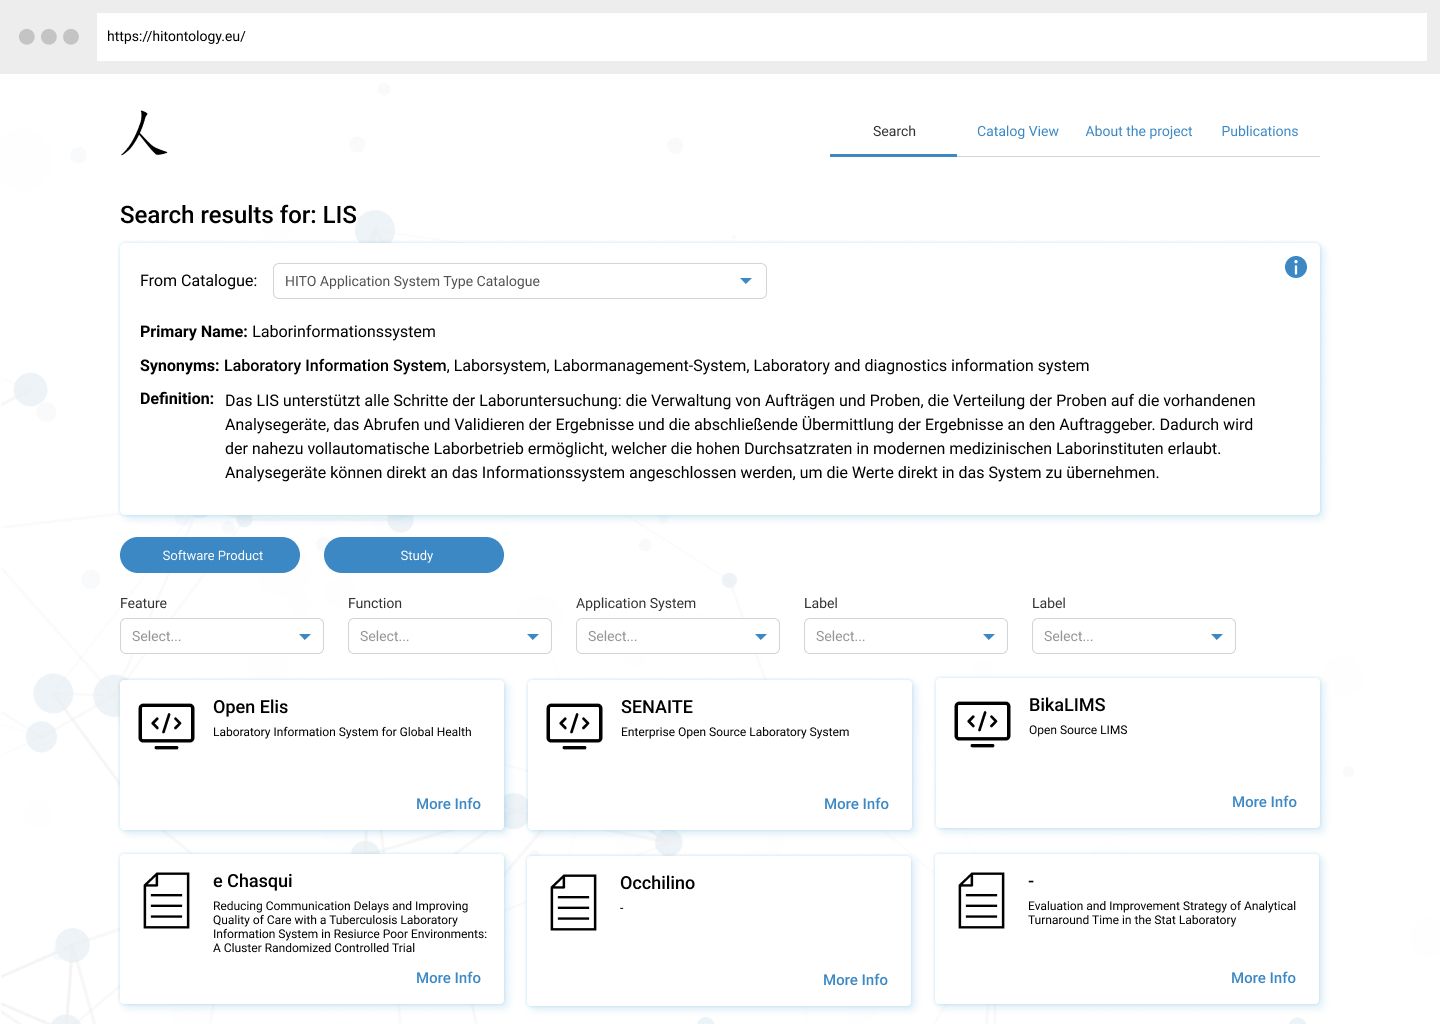
\includegraphics[width=\textwidth]{Images/Mockup_Ergebnisseite}
   	\caption{Mockup - Ergebnisseite}
   	\label{fig:mockup_results}
\end{figure}

\paragraph{Detailseite Softwareprodukt}

Das neue Konzept der Detailseite eines Softwareproduktes stellt die Informationen gruppiert nach Kategorien dar.
Die Abbildung \ref{fig:mockup_sp_detail} zeigt das neue Konzept der Detailseite eines Softwareproduktes.
Die Daten werden in den folgenden vier Gruppen dargestellt:

\begin{itemize}
\item \textbf{General Information:} hier werden allgemeine Merkmale zu einem Softwareprodukt angezeigt.
\item \textbf{Supports Enterprise Function:} hier werden die vom Softwareprodukt unterstütze Unternehmensaufgaben aufgelistet. Die Daten hierfür kommen aus der Beschreibung des Softwareherstellers.
\item \textbf{Offers Feature:} in diesem Fall werden die Funktionen aufgelistet, die das Softwareprodukt anbietet. Auch in diesem Fall kommen die Daten direkt aus der Beschreibung des Softwareproduktes.
\item \textbf{Studies:} hier werden Nutzer über existierende Studien zu dem ausgewählten Softwareprodukt informiert. Hierbei soll über die Beziehung \enquote{evaluates} zwischen Studie und Softwareprodukt untersucht werden, ob  Studien zu dem Softwareprodukt existieren.
\end{itemize}

\begin{figure}[H]
	\centering
    	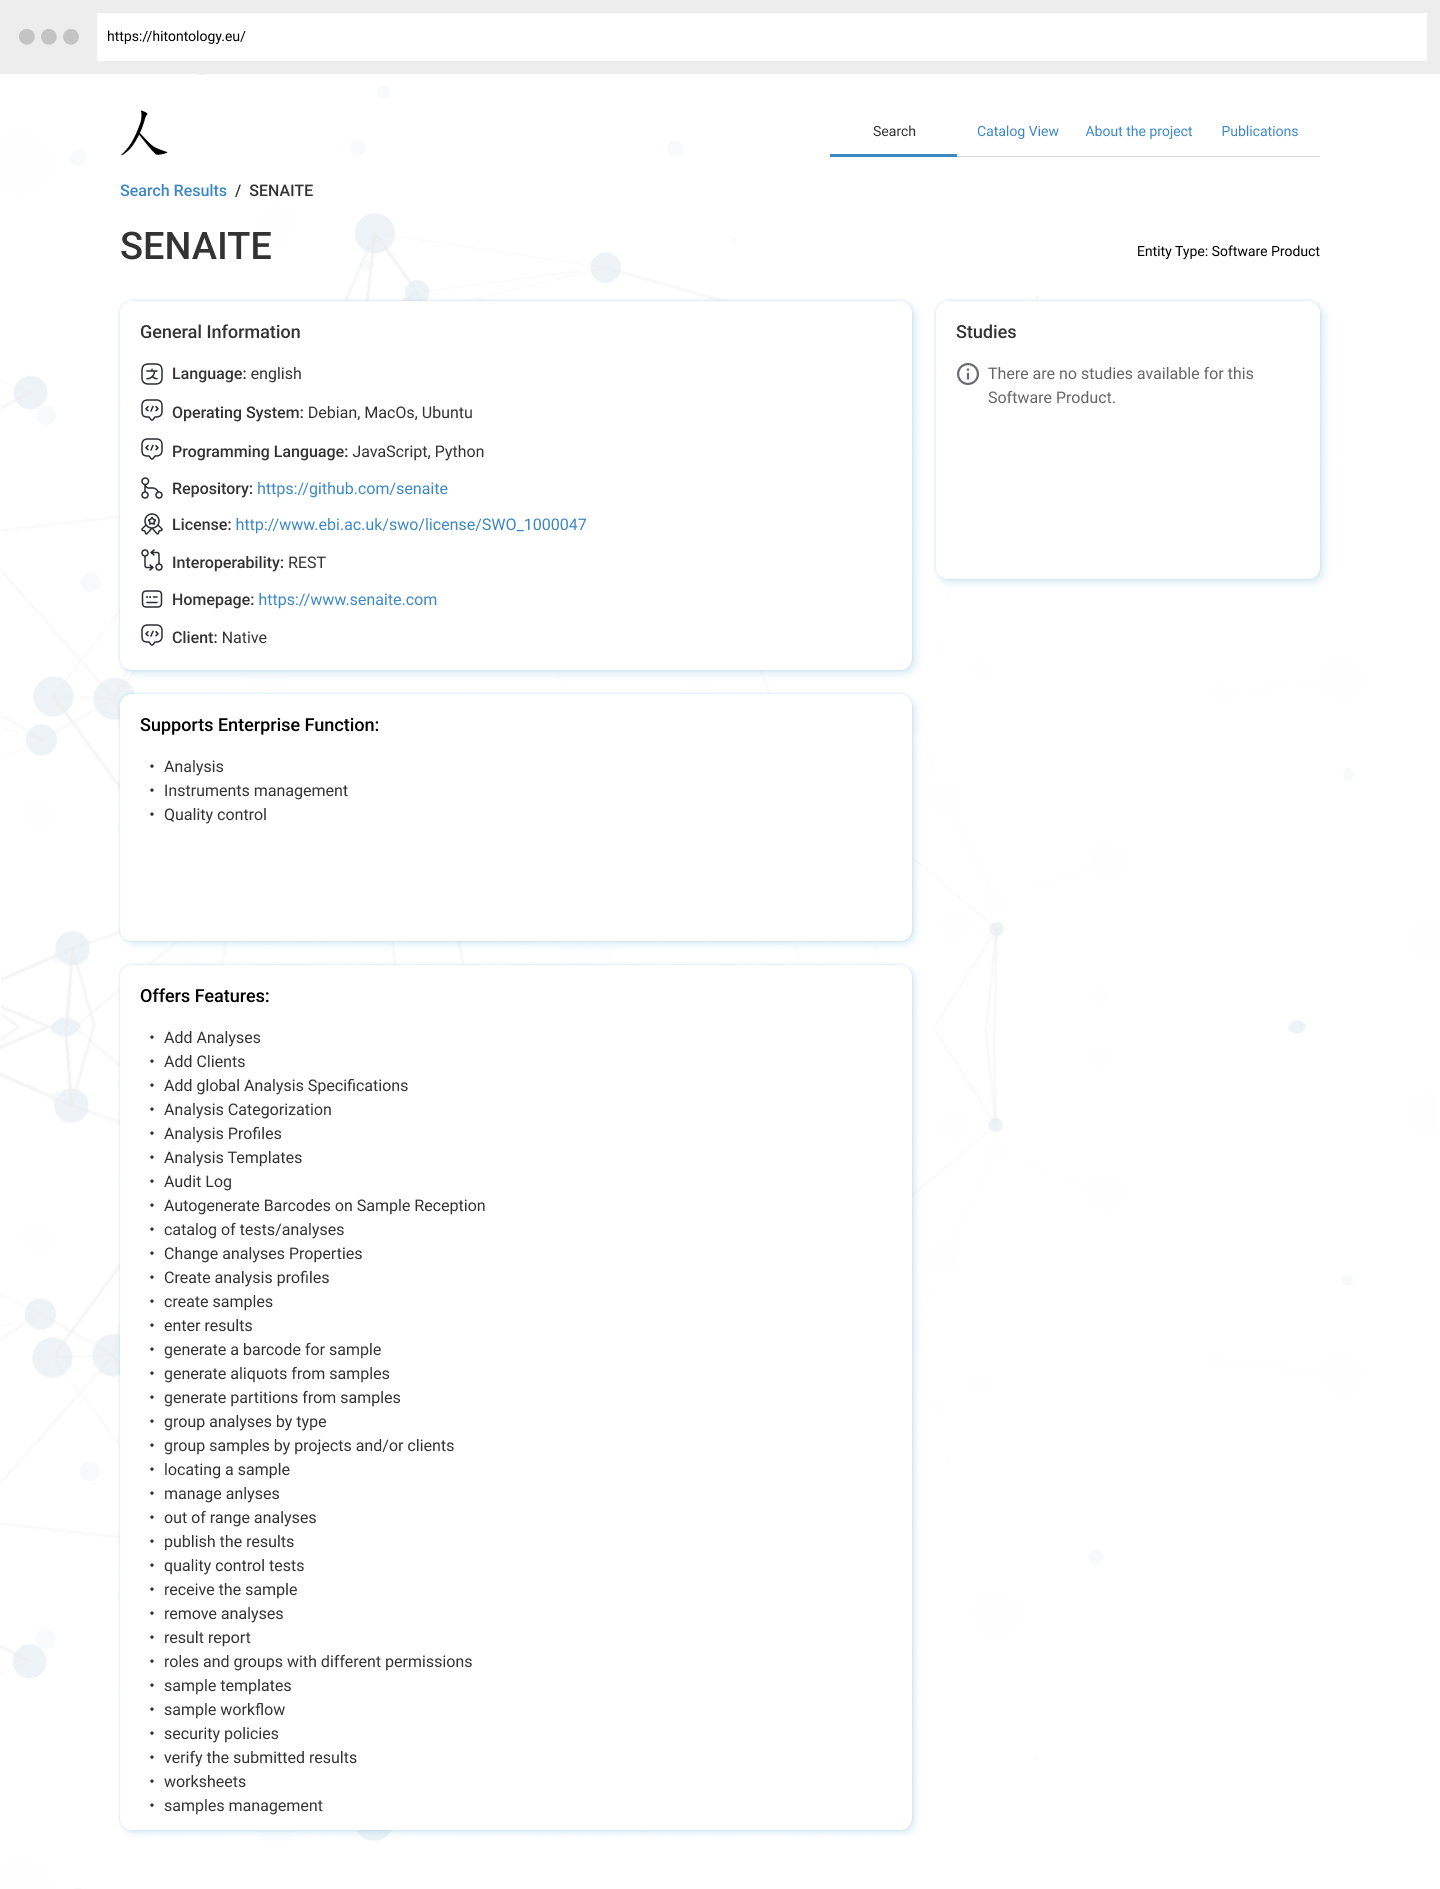
\includegraphics[width=\textwidth]{Images/SP_Detailseite}
   	\caption{Mockup - Detailseite Softwareprodukt}
   	\label{fig:mockup_sp_detail}
\end{figure}

\paragraph{Detailseite Studie}

Das neue Visualisierungskonzept der Detailseite einer Studie ist ähnlich der Detailseite eines Softwareproduktes strukturiert.
Die Abbildung \ref{fig:mockup_sp_detail} zeigt das neue Konzept der Detailseite eines Softwareproduktes.
Die Daten werden in diesem Fall in den folgenden Gruppen dargestellt:

\begin{itemize}
\item \textbf{General Information:} hier werden allgemeine Informationen zu einer Studie dargestellt, wie zum Beispiel wer der Autor der Studie ist oder in welchem Jahr die Studie publiziert wurde.
\item \textbf{Evaluates Application System Type Having Feature Range Shape:} hier werden die vom Softwareprodukt unterstütze Unternehmensaufgaben aufgelistet. Die Daten hierfür kommen aus der Beschreibung des Softwareherstellers.
\item \textbf{Access:} in diesem Fall werden die Funktionen aufgelistet, die das Softwareprodukt anbietet. Auch in diesem Fall kommen die Daten direkt aus der Beschreibung des Softwareproduktes.
\end{itemize}

\begin{figure}[H]
	\centering
    	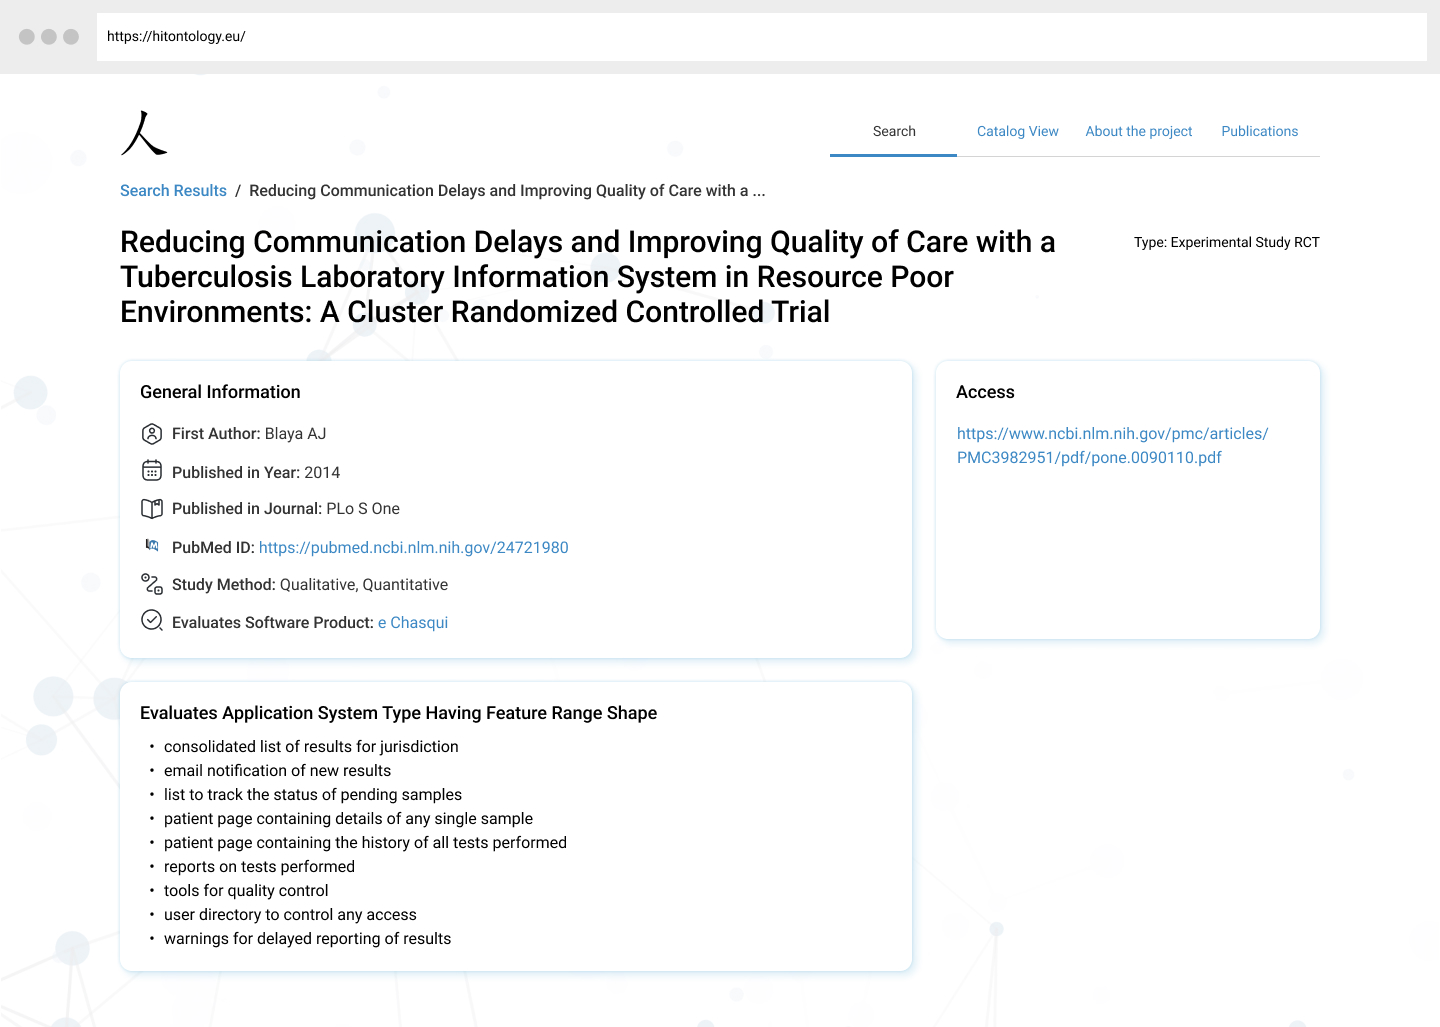
\includegraphics[width=\textwidth]{Images/Studie_Detailseite}
   	\caption{Mockup - Detailseite Studie}
   	\label{fig:mockup_study_detail}
\end{figure}

\paragraph{Katalogübersicht}

Das neue horizontale Menü enthält den Absprung in der Katalogübersicht über den Menüpunkt \enquote{Catalogue View}.
Die Abbildung \ref{fig:mockup_catalogue_overview} zeigt das Konzept der Katalogübersichtseite.
Hier wird ein Überblick über die fünf existierenden Kataloge der Ontologie geschaffen.

\begin{figure}[H]
	\centering
    	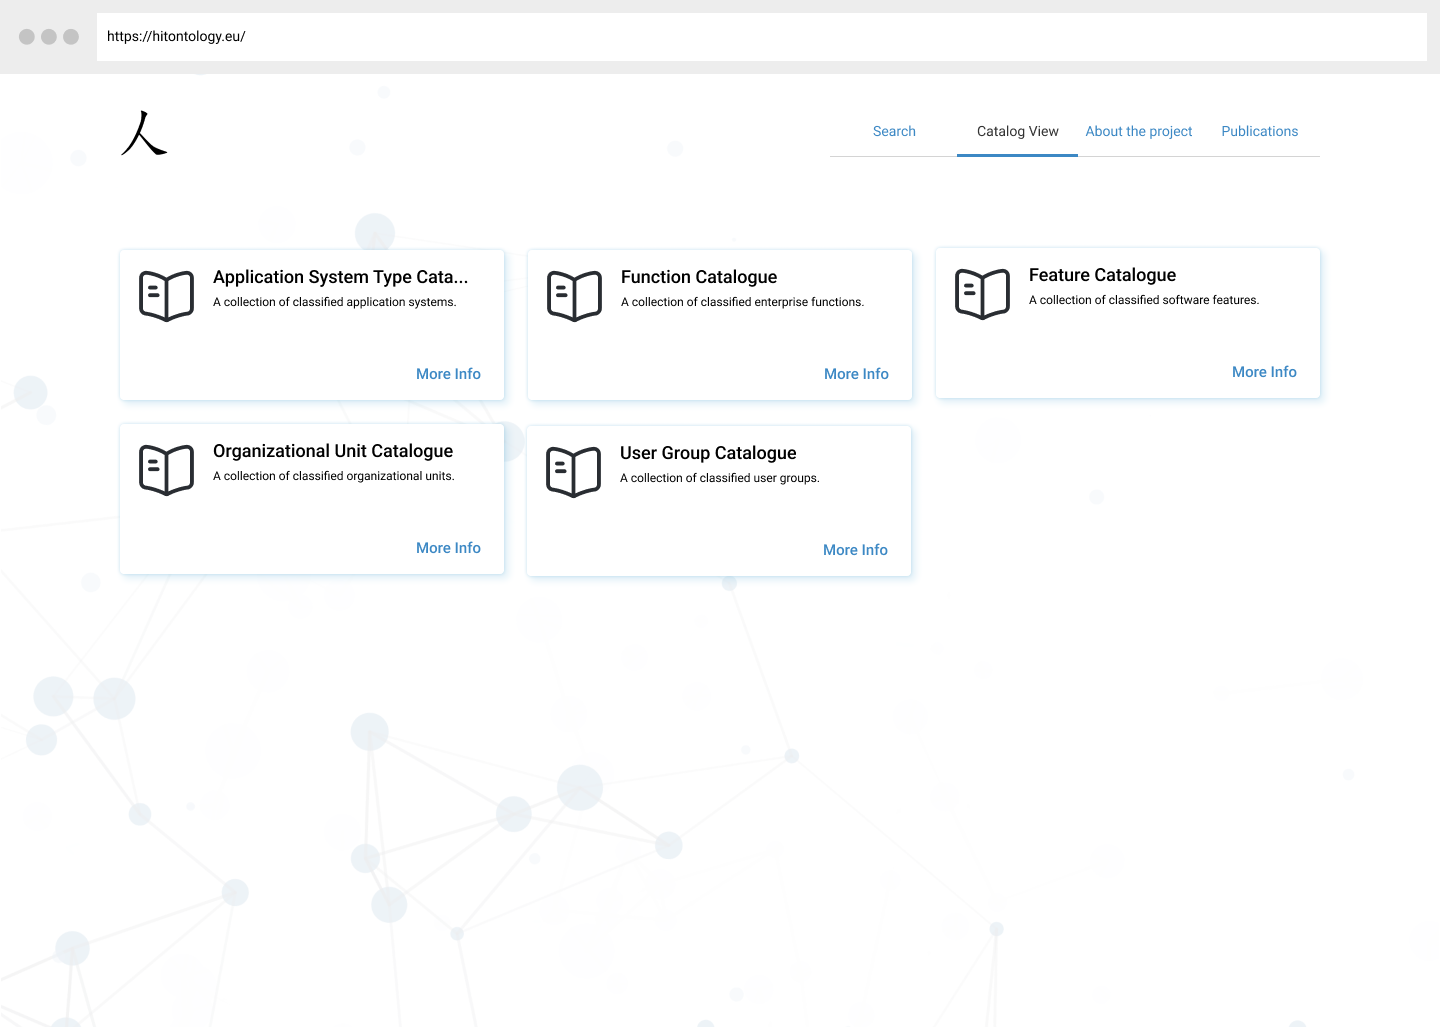
\includegraphics[width=\textwidth]{Images/Katalog_Uebersicht}
   	\caption{Mockup - Katalogübersicht}
   	\label{fig:mockup_catalogue_overview}
\end{figure}

\paragraph{Detailseite Katalog}

Die Detailseite eines Katalogs zeigt auf dem ersten Blick die 
Hier können Nutzer*innen ein Katalog auswählen uns aufklappen.
Die Nutzer*innen können sich dann die Begriffe aus dem ausgewählten Katalog anschauen.
Die Abbildung \ref{fig:mockup_catalogue_detail} zeigt die Detailseite eines Katalogs im nicht ausgeklapptem Zustand und die Abbildung \ref{fig:mockup_catalogue_detail_expanded} zeigt die Detailseite eines Katalogs im ausgeklapptem Zustand.

\begin{figure}[H]
	\centering
    	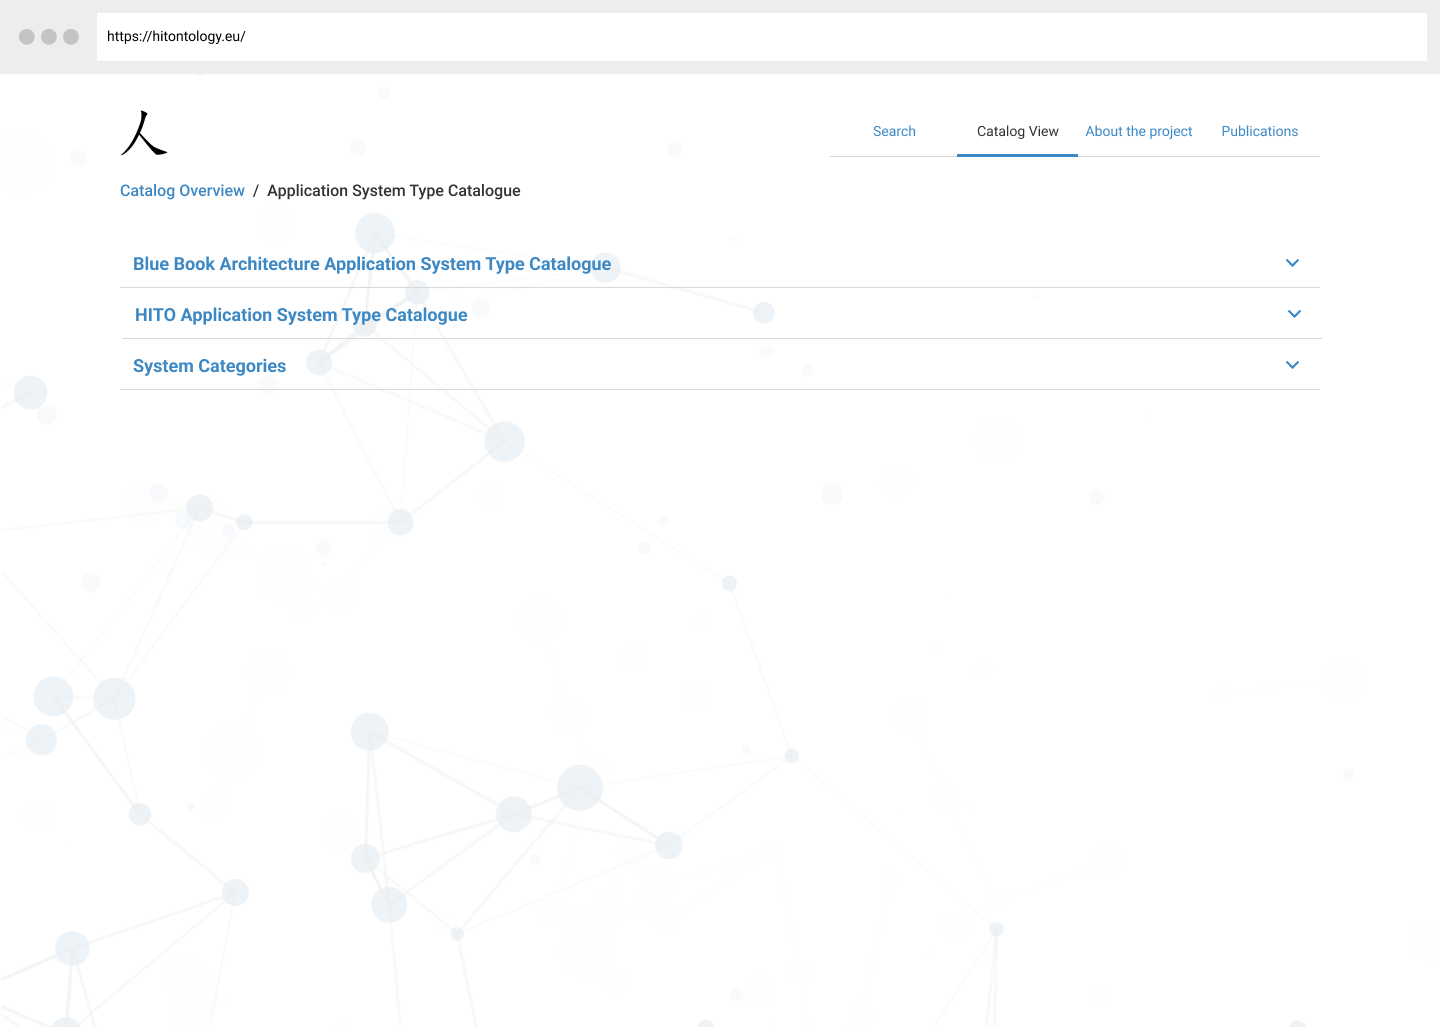
\includegraphics[width=\textwidth]{Images/Katalog_Detailseite}
   	\caption{Mockup - Detailseite Katalog}
   	\label{fig:mockup_catalogue_detail}
\end{figure}

\begin{figure}[H]
	\centering
    	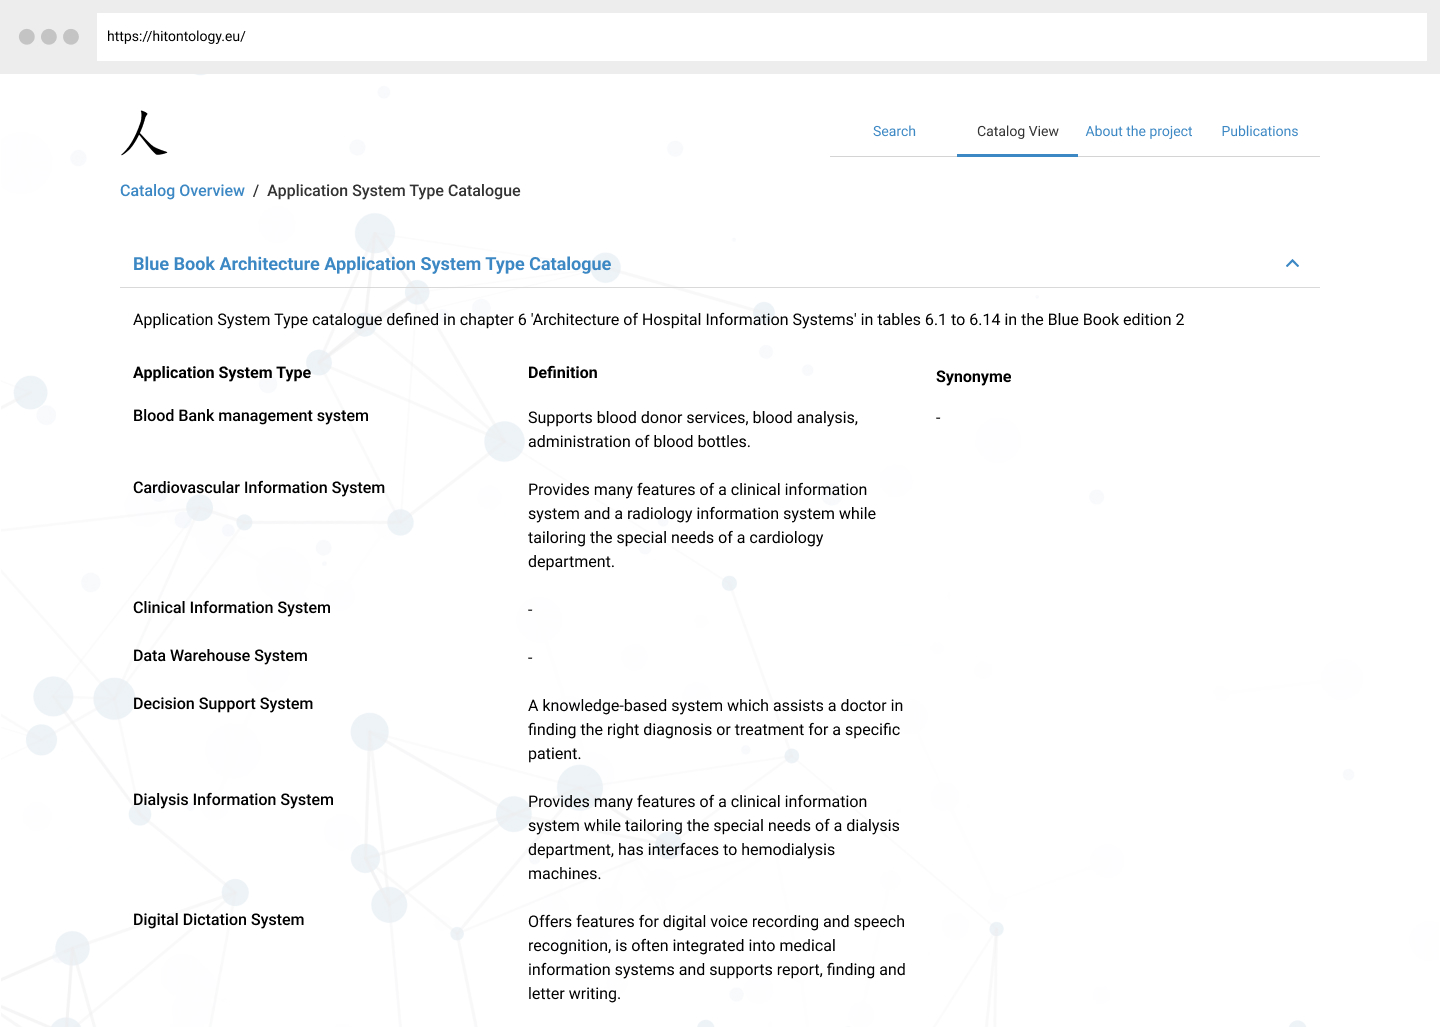
\includegraphics[width=\textwidth]{Images/Katalog_Detailseite_Ausgeklappt}
   	\caption{Mockup - Detailseite Katalog Ausgeklappt}
   	\label{fig:mockup_catalogue_detail_expanded}
\end{figure}

\subsection{Prototyp}

Nach der Erstellung der Mockups, wurde eine Prototyp erstellt.
Dieser wurde ausschließlich zu Präsentationszwecke verwendet und kann unter diesem \href{https://figma.fun/71cjZX}{Link} aufgerufen werden.

\section{Evaluation}

Im letzten Schritt wurde eine finale Evaluation mit Hilfe der Usability Review Technik durchgeführt.
Hierbei wurde das User Interface Design anhand der zehn Heuristiken nach \citet{nielsen_usability_1993} bewertet.
Das Ergebnis der Evaluation soll auf Usability Probleme hinweisen, um diese dann vor der Entwicklung zu beheben.

Im Folgenden werden die zehn Heuristiken anhand der Ergebnisse des neuen User Interface Designs der Anwendung erläutert.
Des Weiteren wird auch Vergleich des vorher und nachher Zustandes gemacht.

\begin{enumerate}
\item \textbf{\enquote{Sichtbarkeit des Systemstatus}} \newline
In diesem Fall geht es darum, dass Nutzer*innen deutlich gemacht wird was die Anwendung in jedem Moment macht und dass jede Aktion des Nutzers mit einer Reaktion der Anwendung 
Hier kann man als Beispiel die Verfeinerung der Ergebnisse anhand der facettierten Suchen nennen.
In der Abbildung \ref{fig:point1_before} sind die Filter auf der linken Seite des Fensters angesetzt.
Wenn ein*e Nutzer*in eine Auswahl trifft, kann er nicht genau sehen, was für eine Reaktion erzeugt wird.
Erst nachdem der/die Nutzer+in wieder nach oben gescrollt hat, kann die gefilterte Ergebnisliste beobachtet werden.
Das Lösung dieses Problems kann in der Abbildung \ref{fig:point_after} beobachtet werden.
Hier befinden sich die Filter über die Ergebnisse, so dass bei der Auswahl eines Filters Nutzer*innen direkt die ausgelöste Reaktion bemerken können.

\begin{figure}[H]
	\centering
    	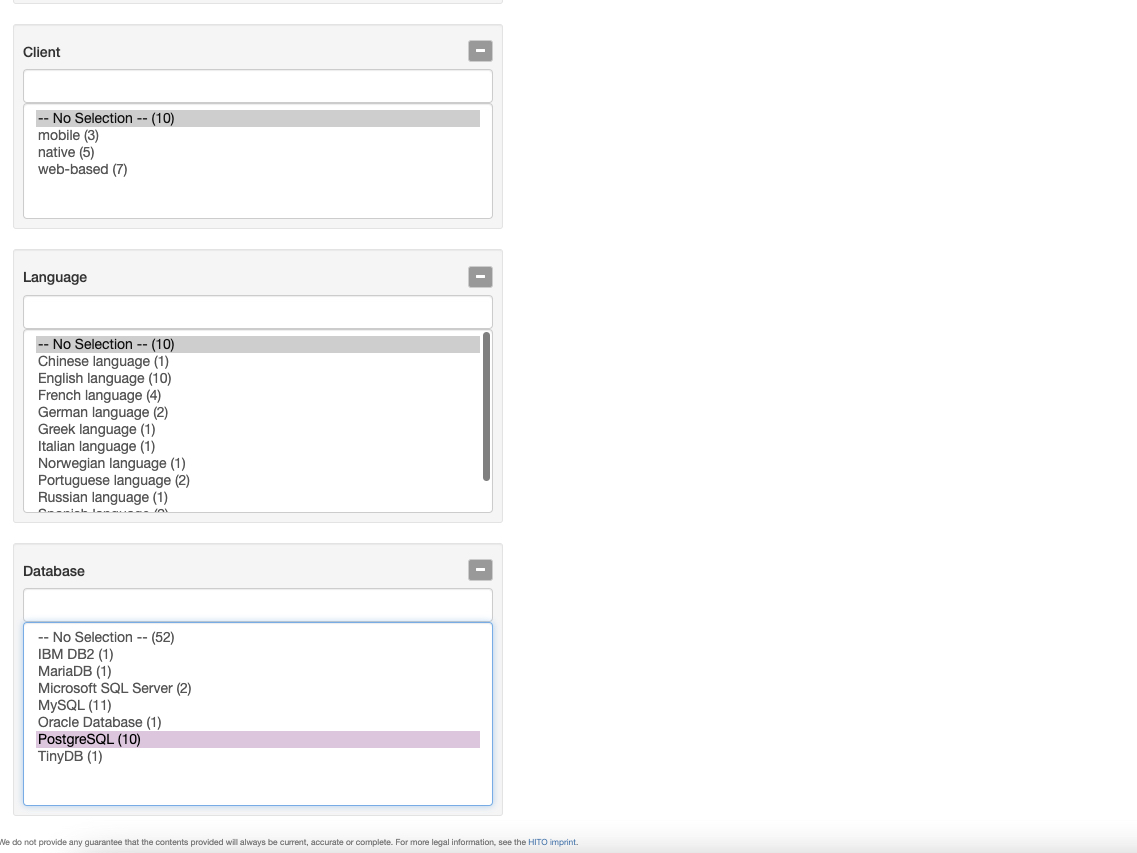
\includegraphics[width=\textwidth]{Images/Punkt_1_davor}
   	\caption{Lösung davor}
   	\label{fig:point1_before}
\end{figure}


\begin{figure}[H]
	\centering
    	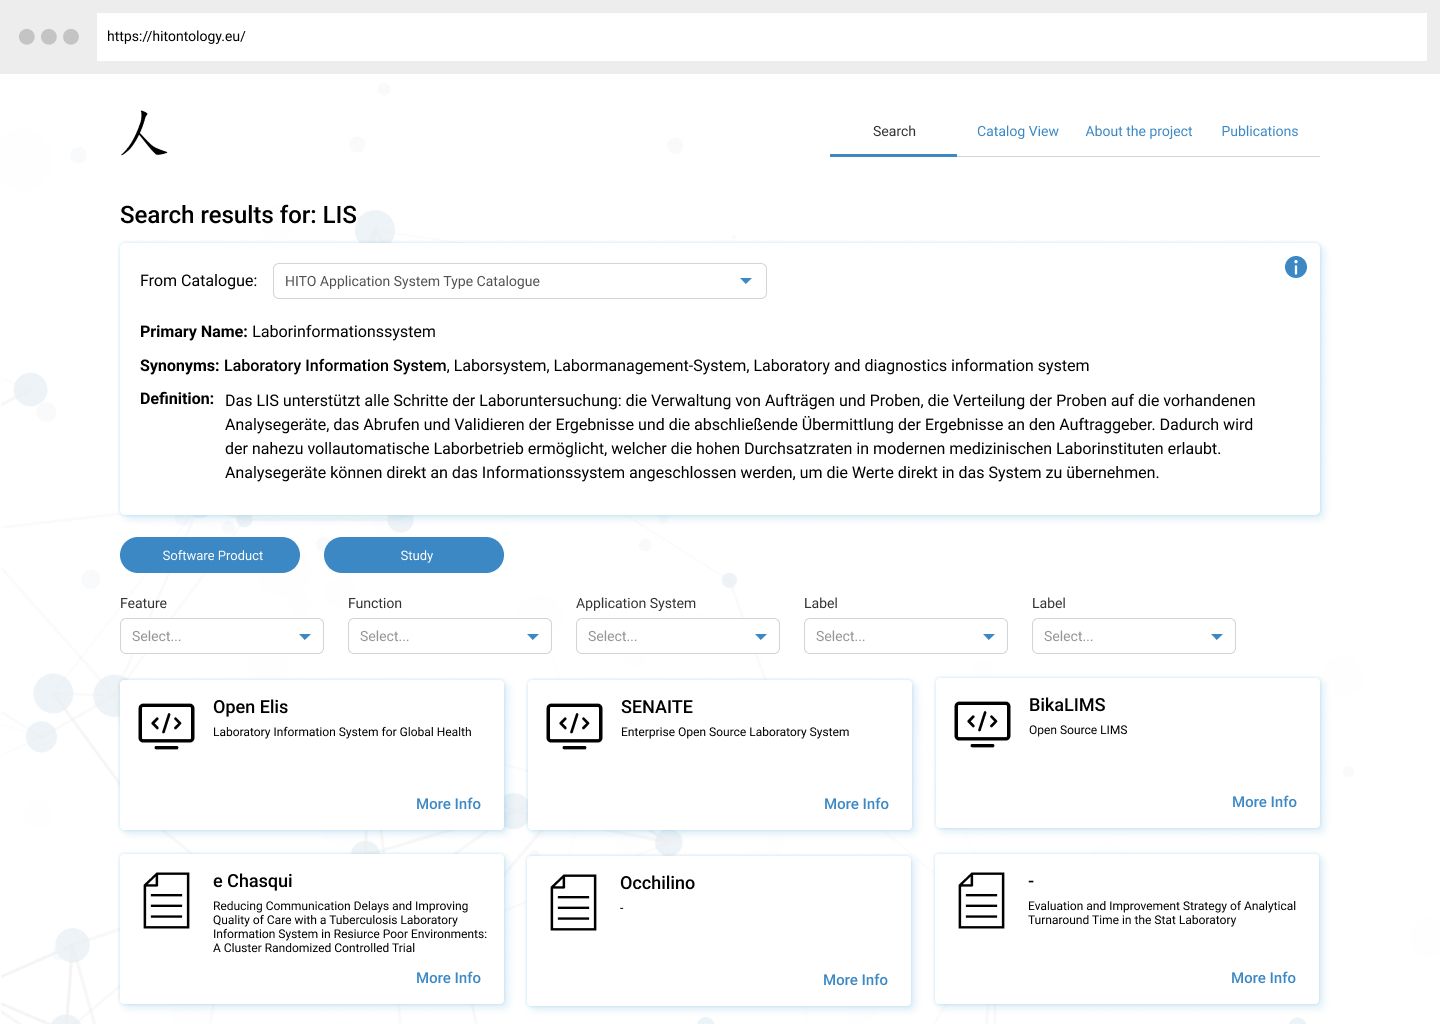
\includegraphics[width=\textwidth]{Images/Mockup_Ergebnisseite}
   	\caption{Lösung danach}
   	\label{fig:point1_after}
\end{figure}


\item \textbf{\enquote{\"Ubereinstimmung von System und die Realität des Nutzers}} \newline
Das User Interface Design soll die Sprache der Nutzer*innen sprechen.
Es sollen nur Begriffe und Konzepte benutzt werden, die dem Wissensstand der Zielgruppe entspricht.
Die Abbildung \ref{fig:point2_before} zeigt den aktuellen Stand der Anwendung.
Hier ist zu beobachten, dass die dargestellten Informationen ohne Formatierung aus der Ontologie übernommen wurden.
Somit ist diese Lösung für die drei Zielgruppen ungeeignet, da diese eine gewisse Einarbeitungszeit in Themen des Semantic Webs erfordert.
Die Abbildung \ref{fig:point2_after} zeigt das neue Konzept des User Interface Designs für die selbe Seite aus der Abbildung \ref{fig:point2_before}.
Hier ist zu beobachten, dass die dargestellten Informationen für Menschen lesbar und verständlich sind.
Weiterhin unterstützen Icons und die Aufteilung der Daten in unterschiedliche Gruppen die Erhöhung des Wiedererkennungswertes auf Seiten mit ähnlichem Aufbau.

\begin{figure}[H]
	\centering
    	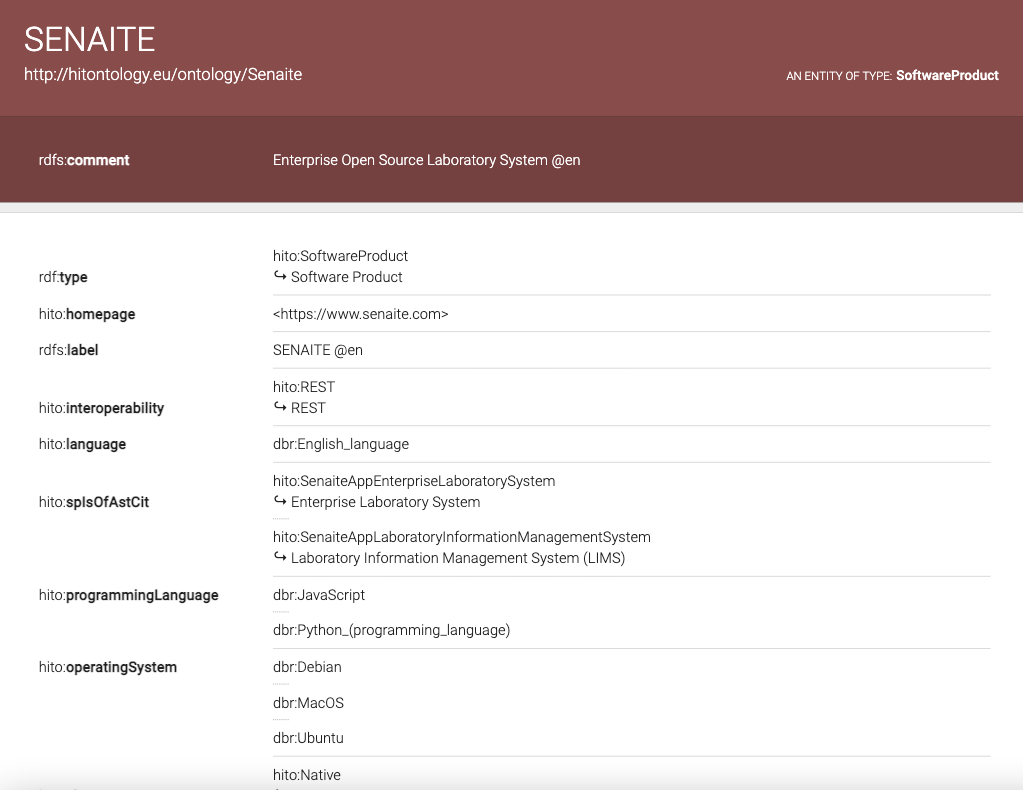
\includegraphics[width=\textwidth]{Images/Punkt_2_davor}
   	\caption{Lösung davor}
   	\label{fig:point2_before}
\end{figure}

\clearpage

\begin{figure}[H]
	\centering
    	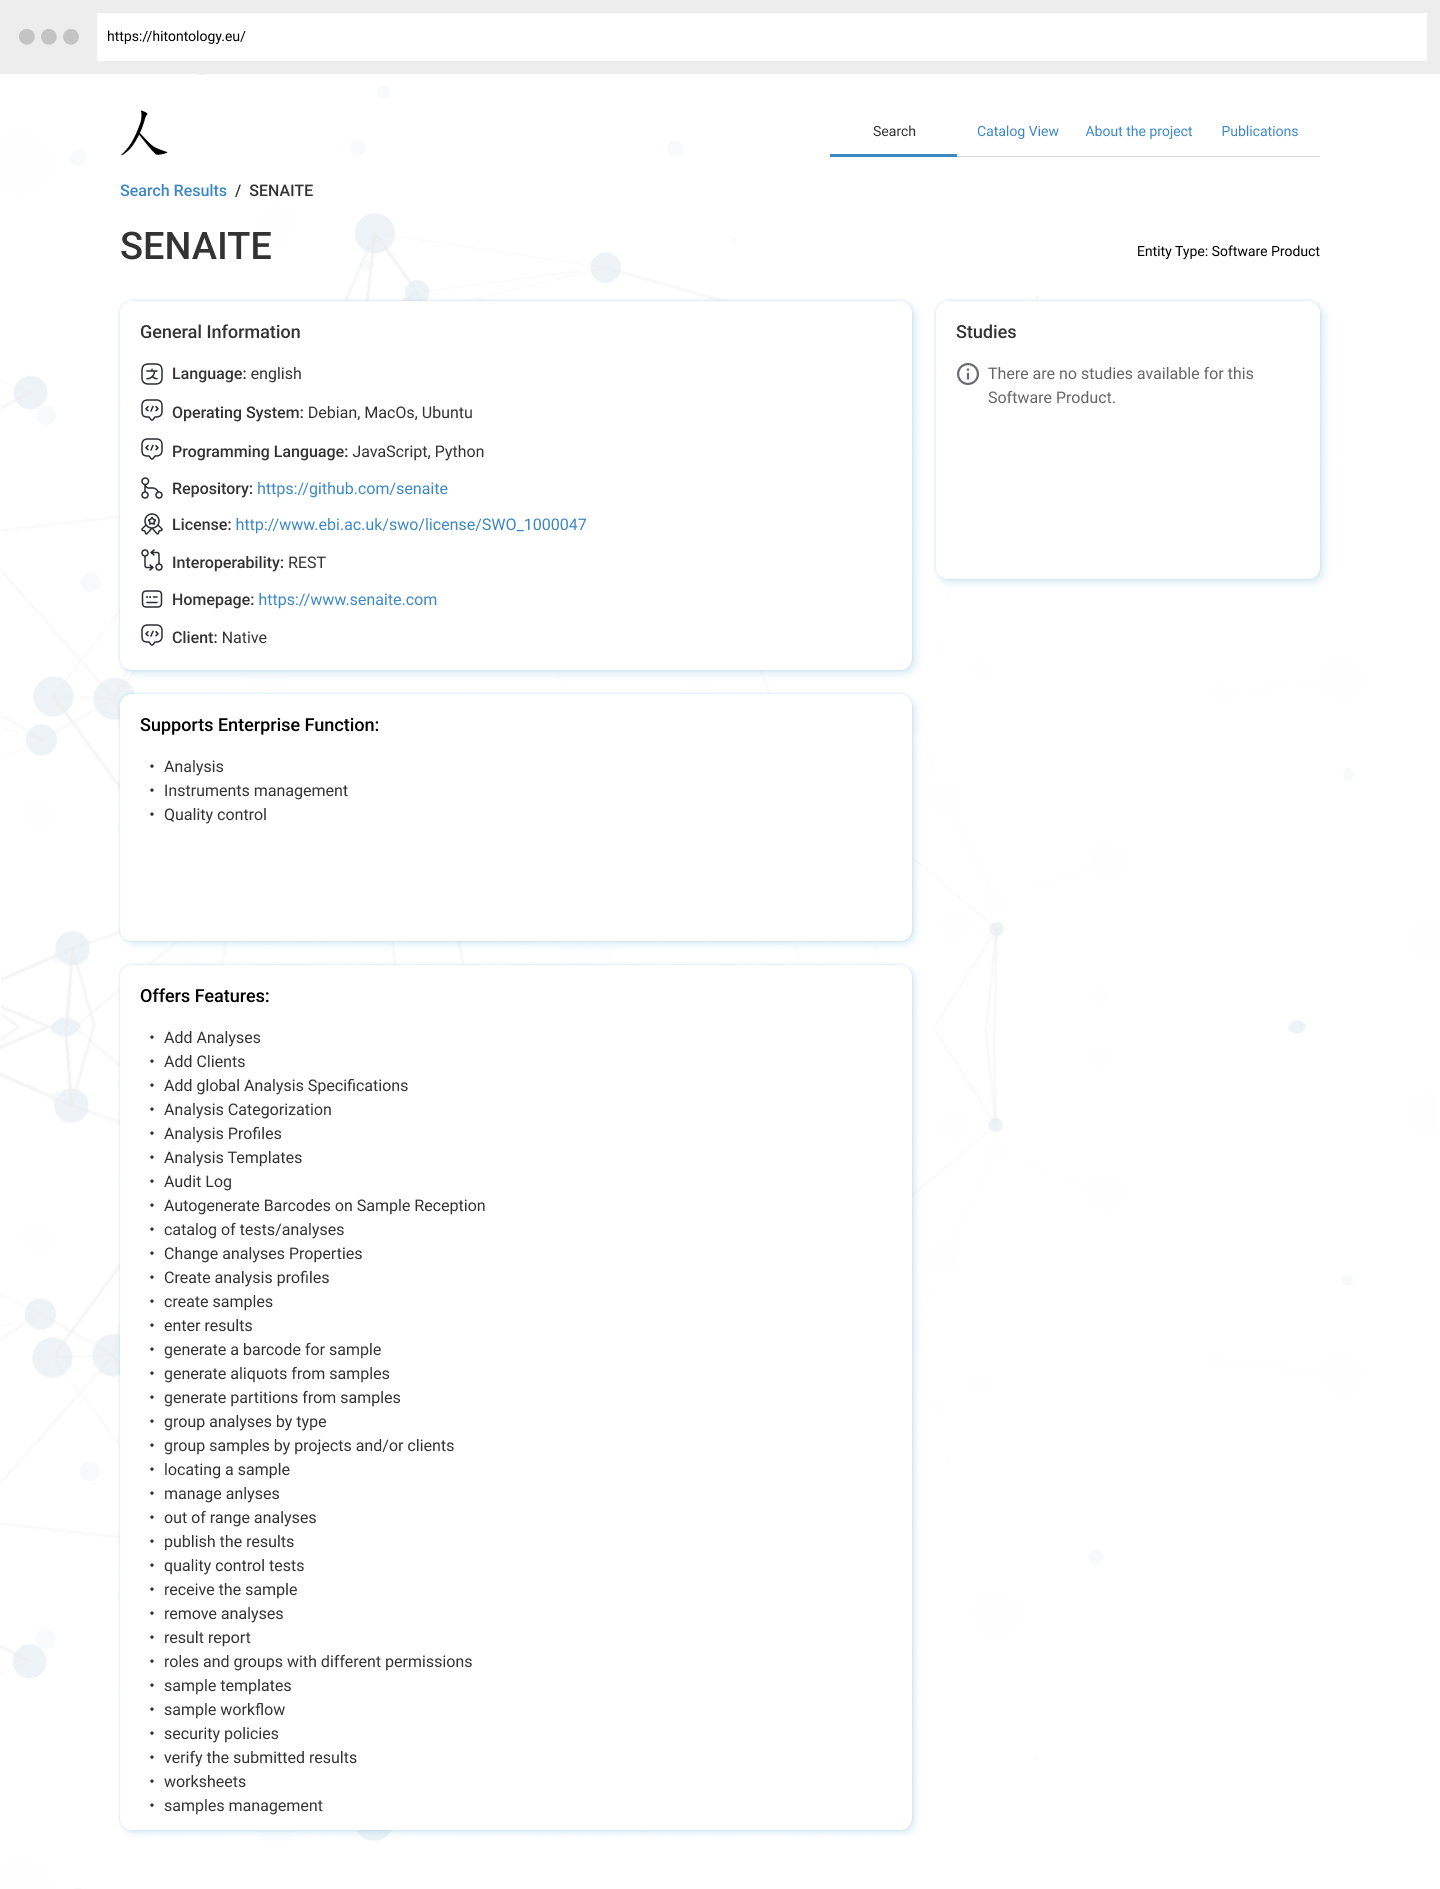
\includegraphics[width=\textwidth]{Images/SP_Detailseite}
   	\caption{Lösung danach}
   	\label{fig:point2_after}
\end{figure}

\clearpage

\item \textbf{\enquote{Kontrolle durch den Nutzer}} \newline

Nutzer*innen führen manchmal Aktionen aus Versehen aus. 
Aus diesem Grund ist es wichtig Wege zum vorherigen Zustand deutlich zu machen.
Das verleiht Nutzer*innen das Gefühl von Kontrolle über die genutzte Anwendung und vermeidet Gefühle wie zum Beispiel Frust seitens der Nutzer*innen.
In dem vorliegenden Fall haben Nutzer*innen keine Möglichkeit zwischen den Unterseiten der Anwendung zu wechseln.
Sie müssen immer zurück zur Startseite (Abbildung \ref{fig:point3_davor}), um auf eine andere Unterseite navigieren zu können.
Für das neue Konzept wurde eine horizontales Menu gedacht, was die Navigation zwischen den Unterseiten erleichtert.
Weiterhin wurden für Detailseiten Breadcrumb Menus verwendet, so dass Nutzer*innen zu der vorherigen Seite wieder springen könnne.

\begin{figure}[H]
	\centering
    	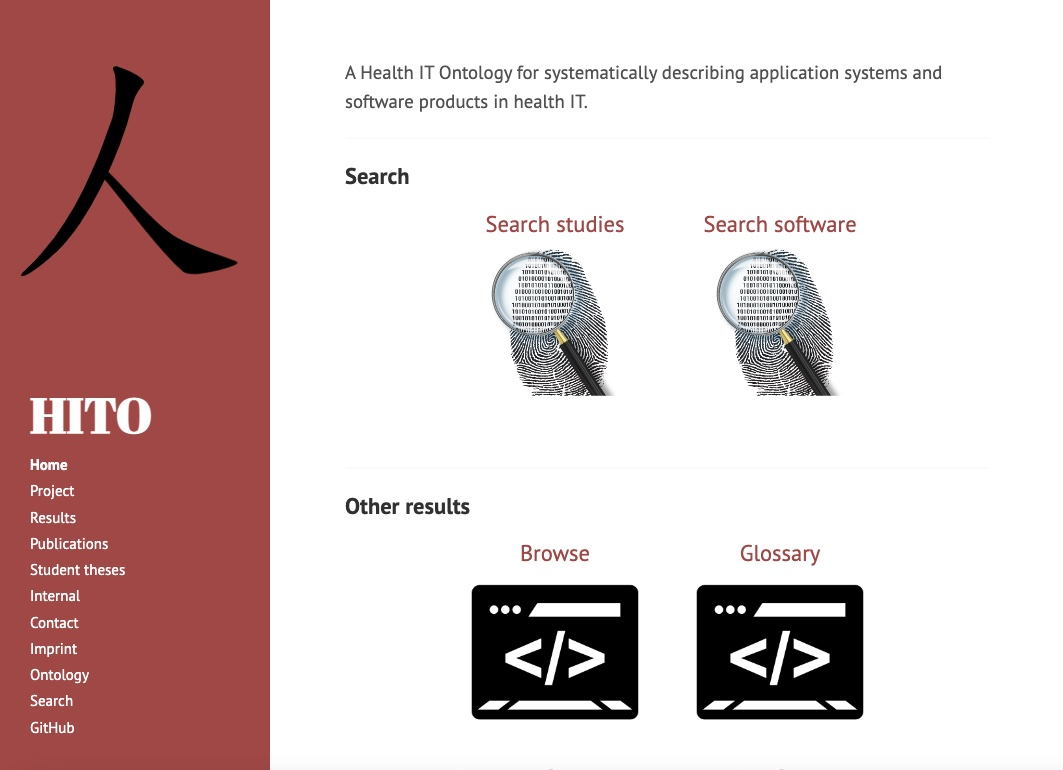
\includegraphics[width=\textwidth]{Images/Punkt_3_davor}
   	\caption{Lösung davor}
   	\label{fig:point3_davor}
\end{figure}

\begin{figure}[H]
	\centering
    	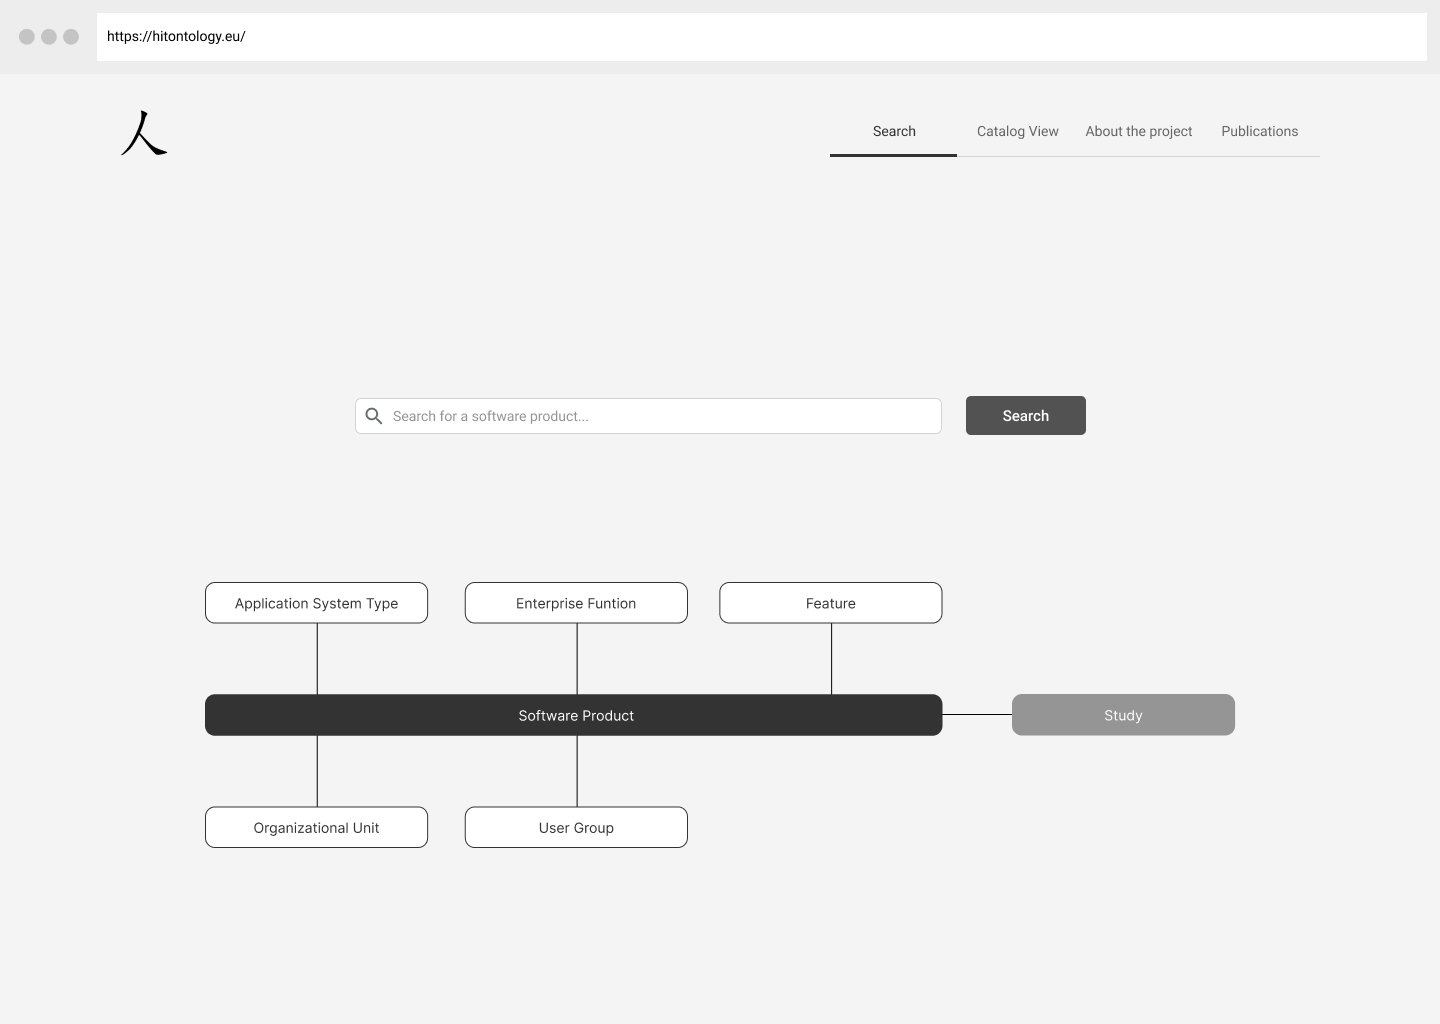
\includegraphics[width=1.45\textwidth, angle=-90]{Images/Startseite}
   	\caption{Lösung danach}
   	\label{fig:wireframe_start}
\end{figure}

\item \textbf{\enquote{Konsistenz und Standards}} \newline

Elemente der Benutzeroberfläche sollen durchgehend ein einheitliches Erscheinungsbild haben.
Sie dürfen nicht unterschiedlich aussehen, wenn sie den selben Zweck erfüllen.
In diesem Fall sollen platform- und industriespezifische Konventionen beachtet werden.
(Hier fehlt noch ein Beispiel)

\begin{figure}[H]
	\centering
    	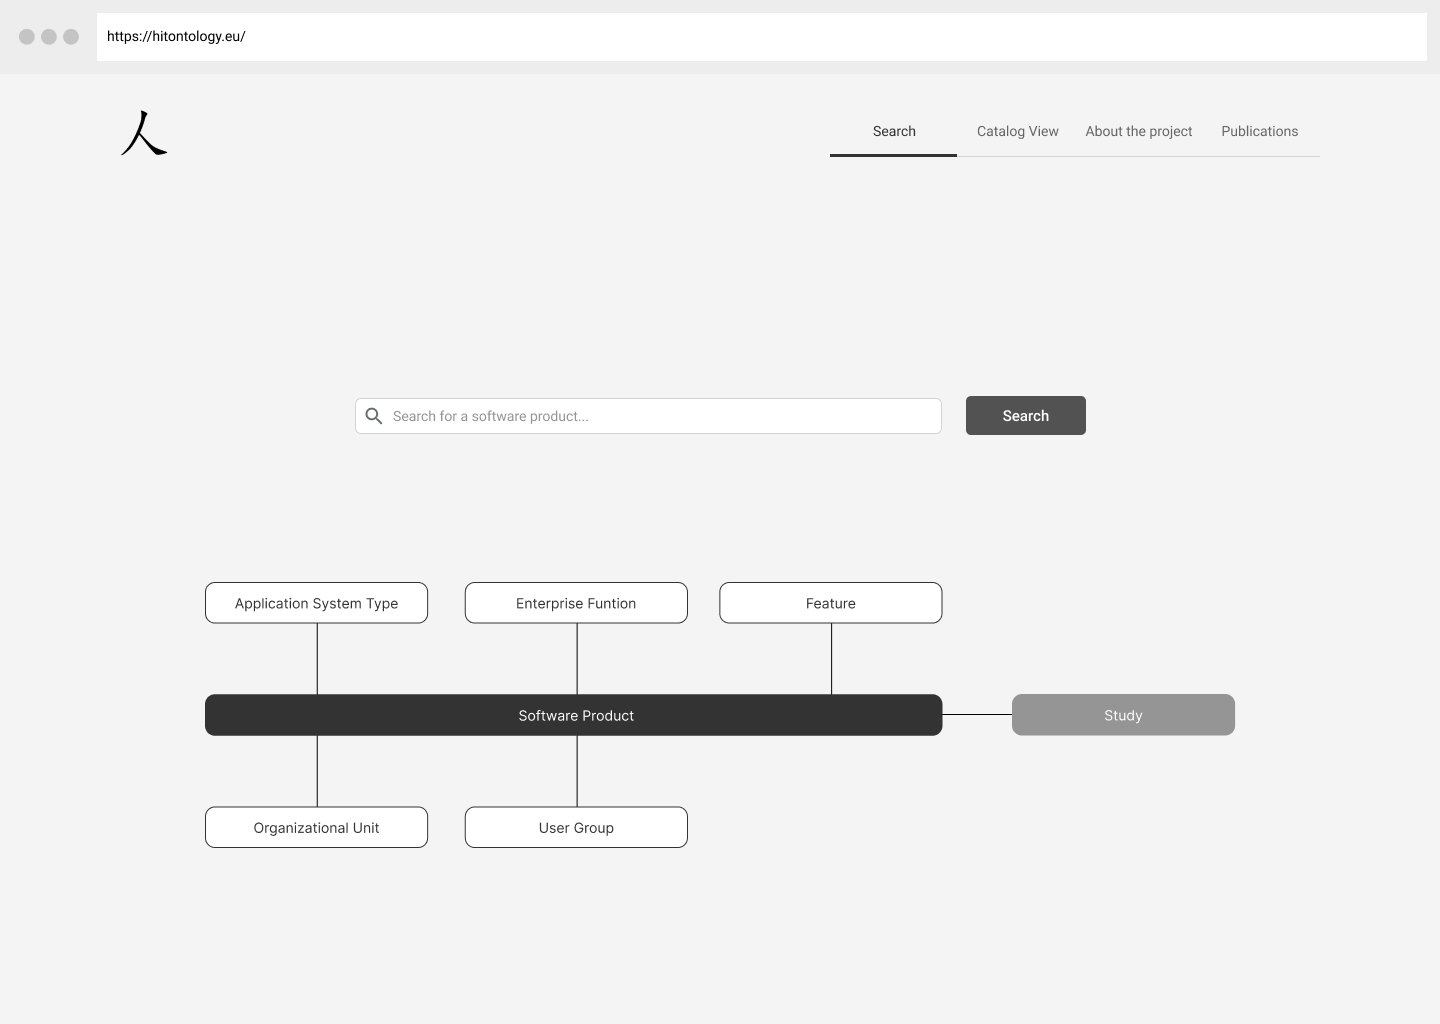
\includegraphics[width=1.45\textwidth, angle=-90]{Images/Startseite}
   	\caption{Lösung davor}
   	\label{fig:wireframe_start}
\end{figure}

\begin{figure}[H]
	\centering
    	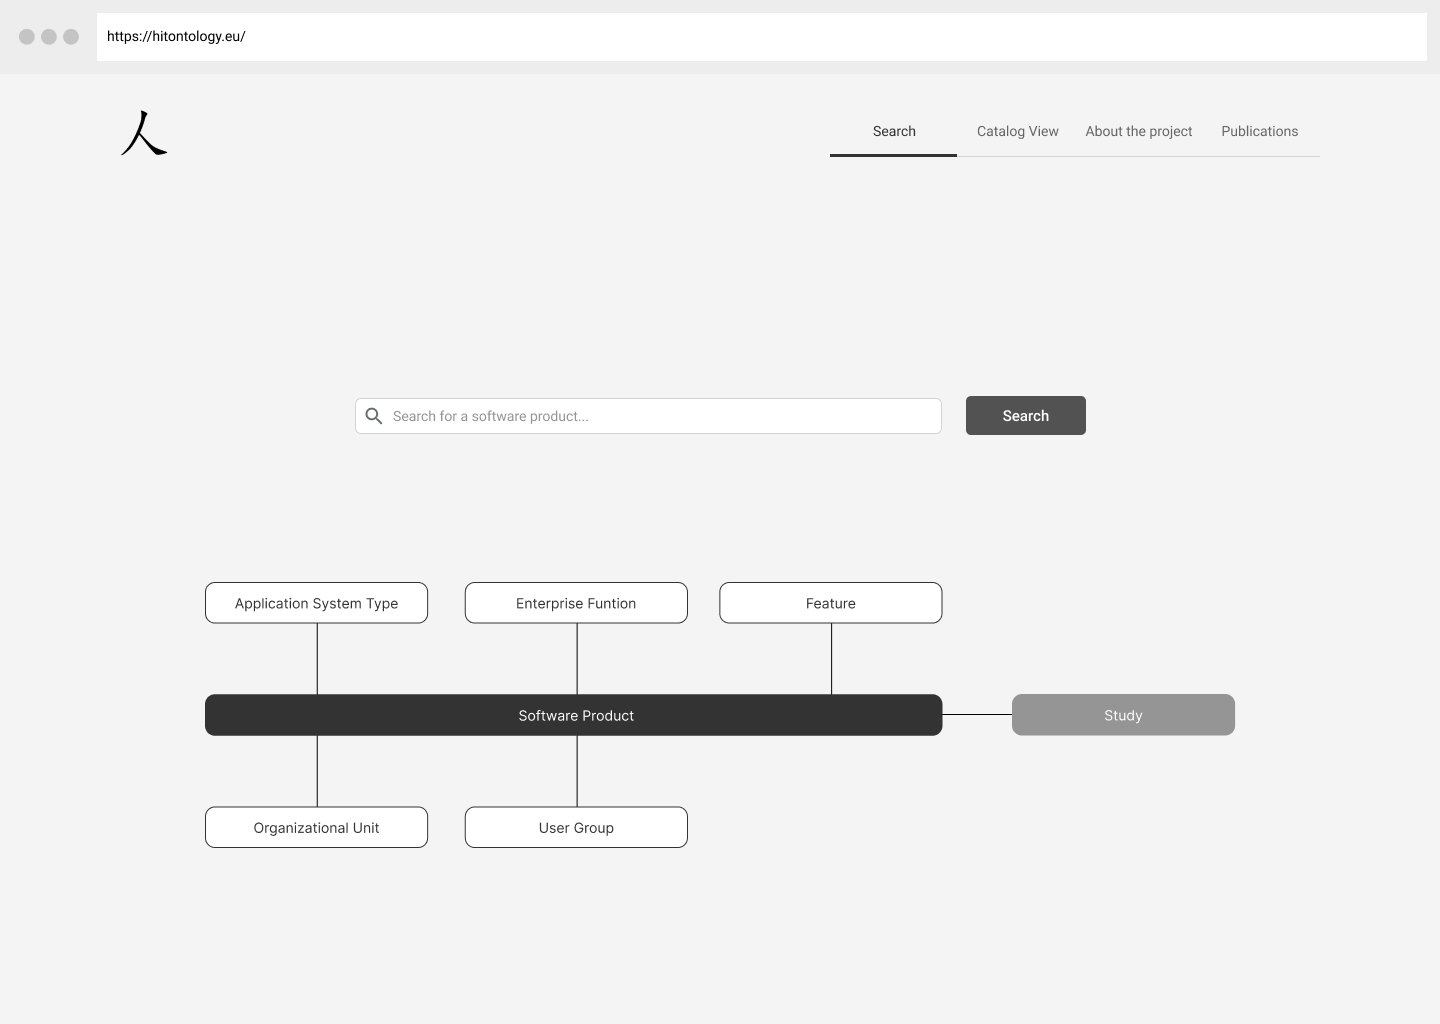
\includegraphics[width=1.45\textwidth, angle=-90]{Images/Startseite}
   	\caption{Lösung danach}
   	\label{fig:wireframe_start}
\end{figure}

\item \textbf{\enquote{Fehlervermeidung}} \newline



\begin{figure}[H]
	\centering
    	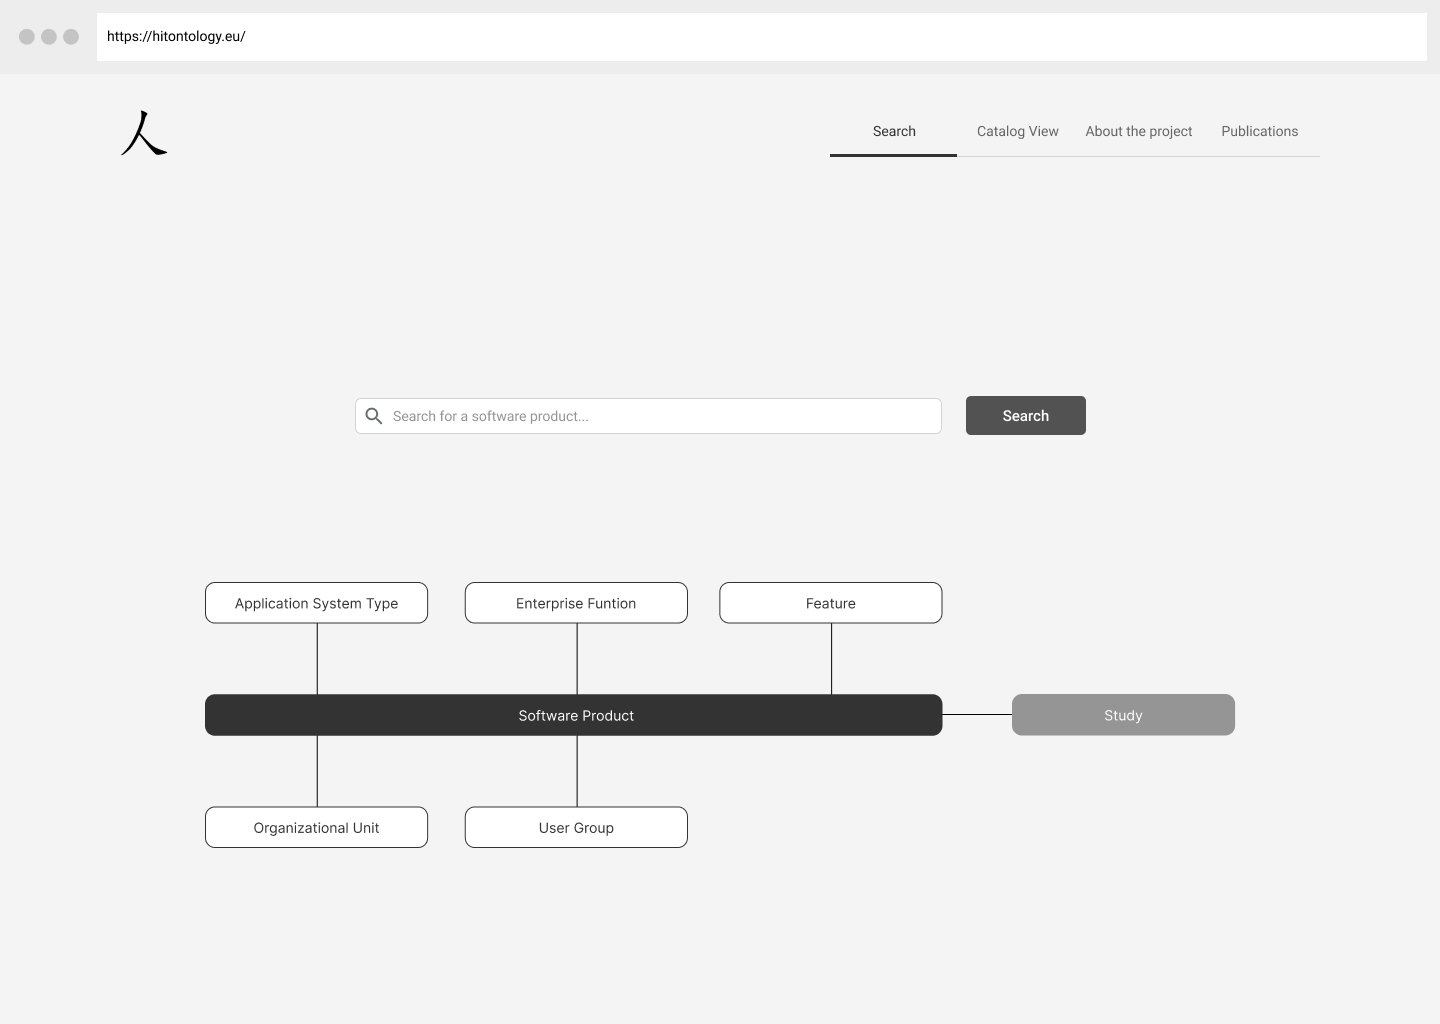
\includegraphics[width=1.45\textwidth, angle=-90]{Images/Startseite}
   	\caption{Lösung davor}
   	\label{fig:wireframe_start}
\end{figure}

\clearpage

\begin{figure}[H]
	\centering
    	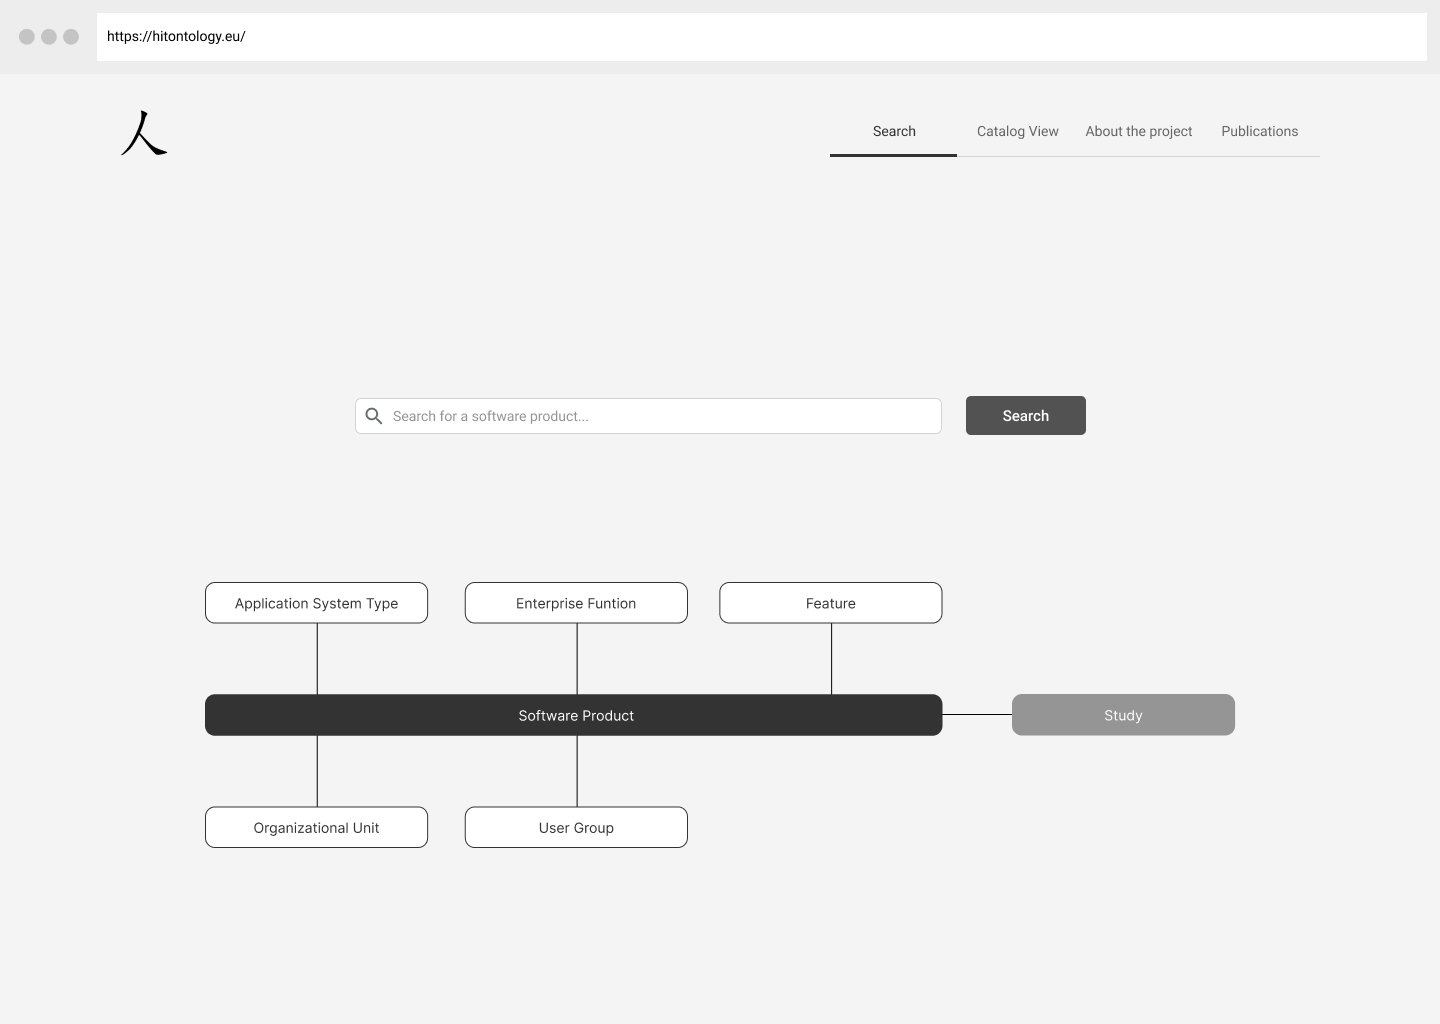
\includegraphics[width=1.45\textwidth, angle=-90]{Images/Startseite}
   	\caption{Lösung danach}
   	\label{fig:wireframe_start}
\end{figure}

\clearpage

\item \textbf{\enquote{Selbsterklärung vor Erinnerung}} \newline

Beispiel hier Anzeige des Suchbegriffes, so dass der Nutzer immer weiß nach welchem Begriff er genau gesucht hat.

\begin{figure}[H]
	\centering
    	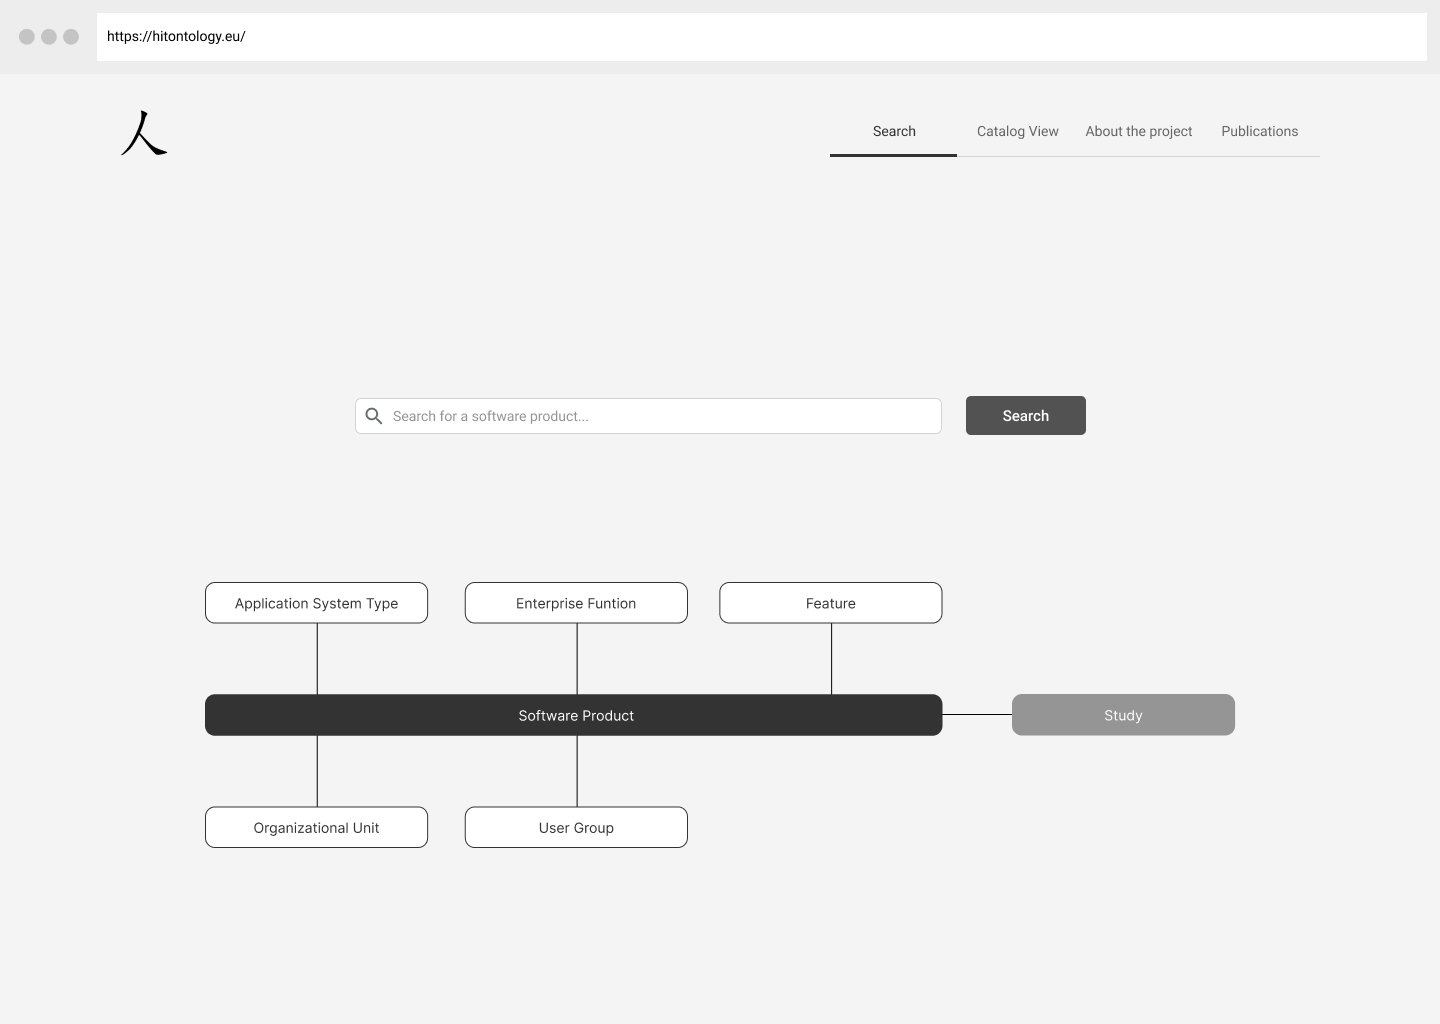
\includegraphics[width=1.45\textwidth, angle=-90]{Images/Startseite}
   	\caption{Lösung davor}
   	\label{fig:wireframe_start}
\end{figure}

\clearpage

\begin{figure}[H]
	\centering
    	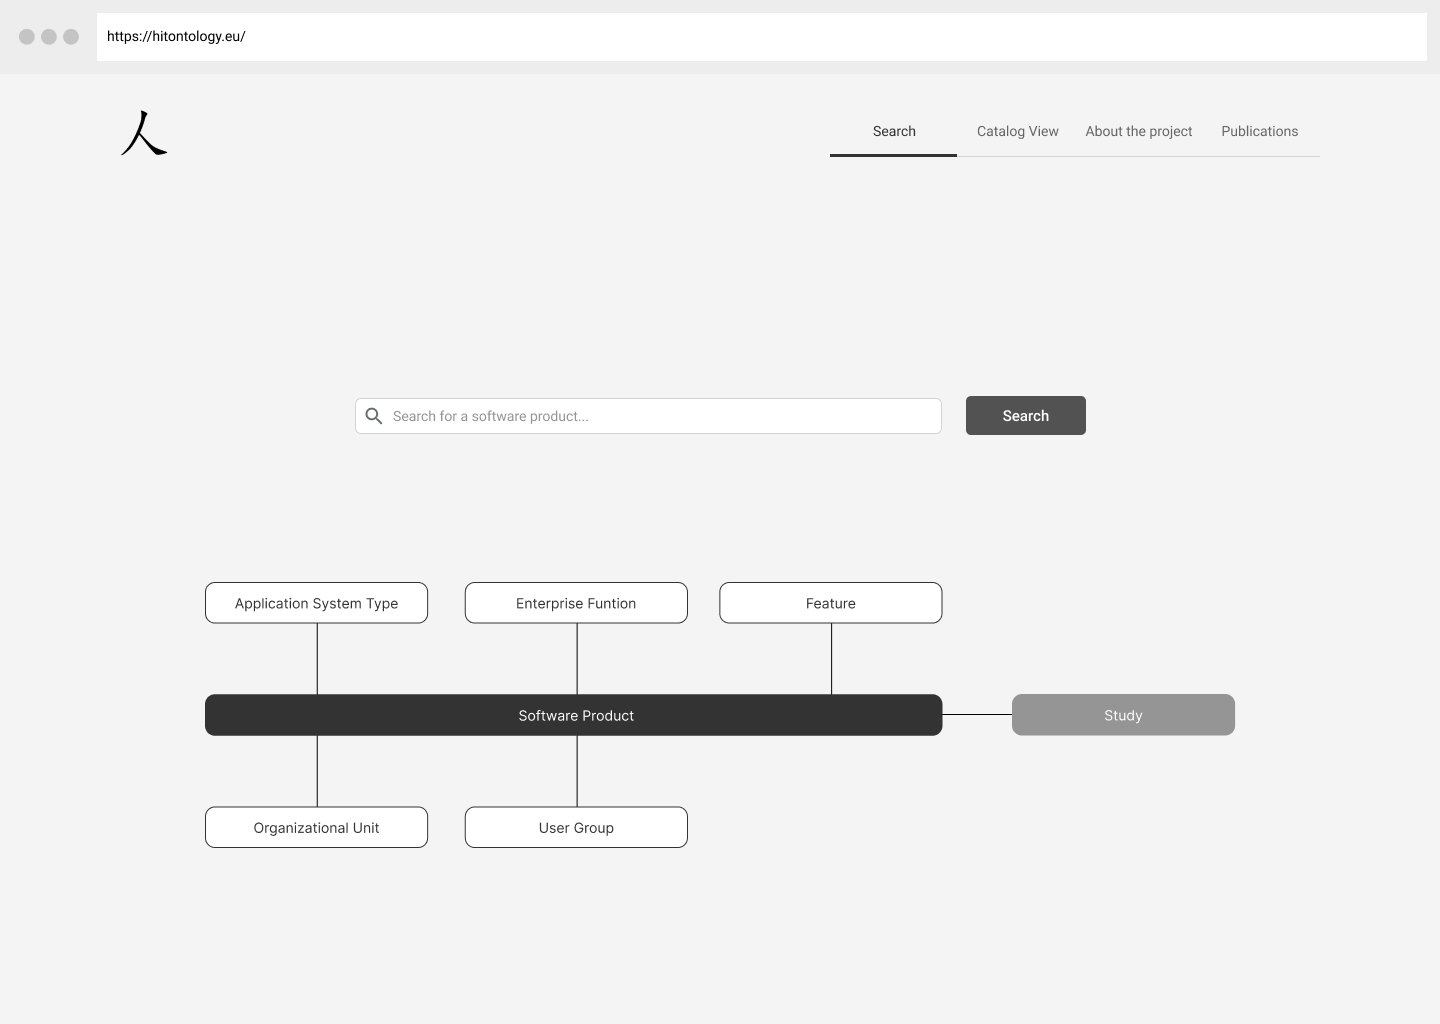
\includegraphics[width=1.45\textwidth, angle=-90]{Images/Startseite}
   	\caption{Lösung danach}
   	\label{fig:wireframe_start}
\end{figure}

\clearpage

\item \textbf{\enquote{Flexibilität und Effizienz}} \newline
Hier als Beispiel Katalogübersicht
Hier Erklärung der Heuristik + Darstellung des bevor- und danach-Zustandes. 
Lorem ipsum dolor sit amet, consetetur sadipscing elitr, sed diam nonumy eirmod tempor invidunt ut labore et dolore magna aliquyam erat, sed diam voluptua.

\begin{figure}[H]
	\centering
    	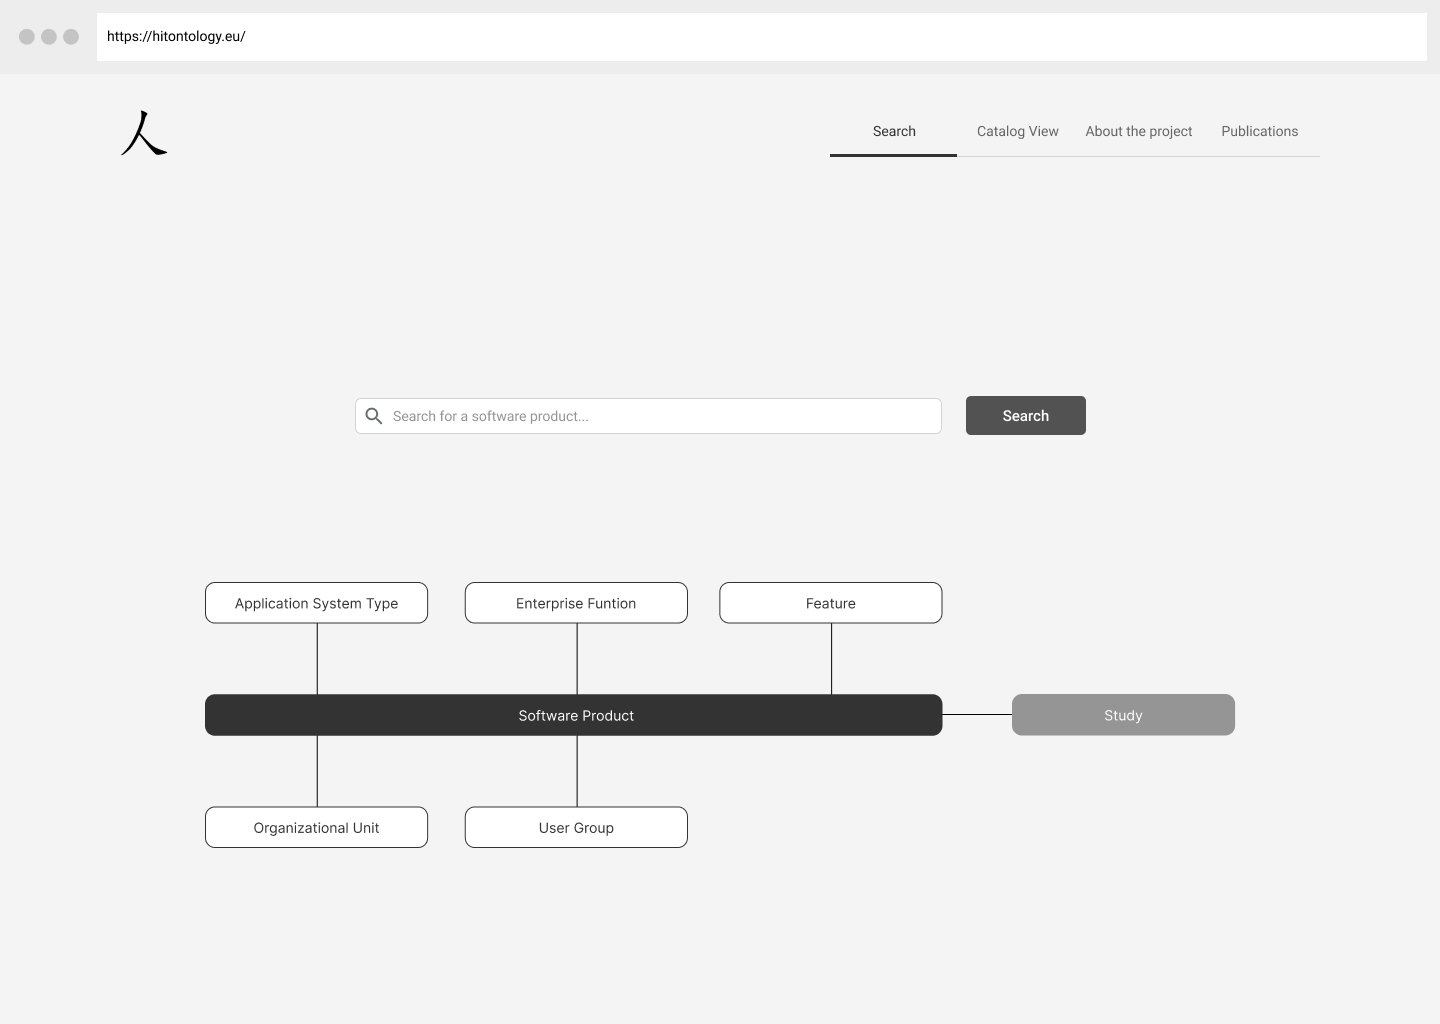
\includegraphics[width=1.45\textwidth, angle=-90]{Images/Startseite}
   	\caption{Lösung davor}
   	\label{fig:wireframe_start}
\end{figure}

\clearpage

\begin{figure}[H]
	\centering
    	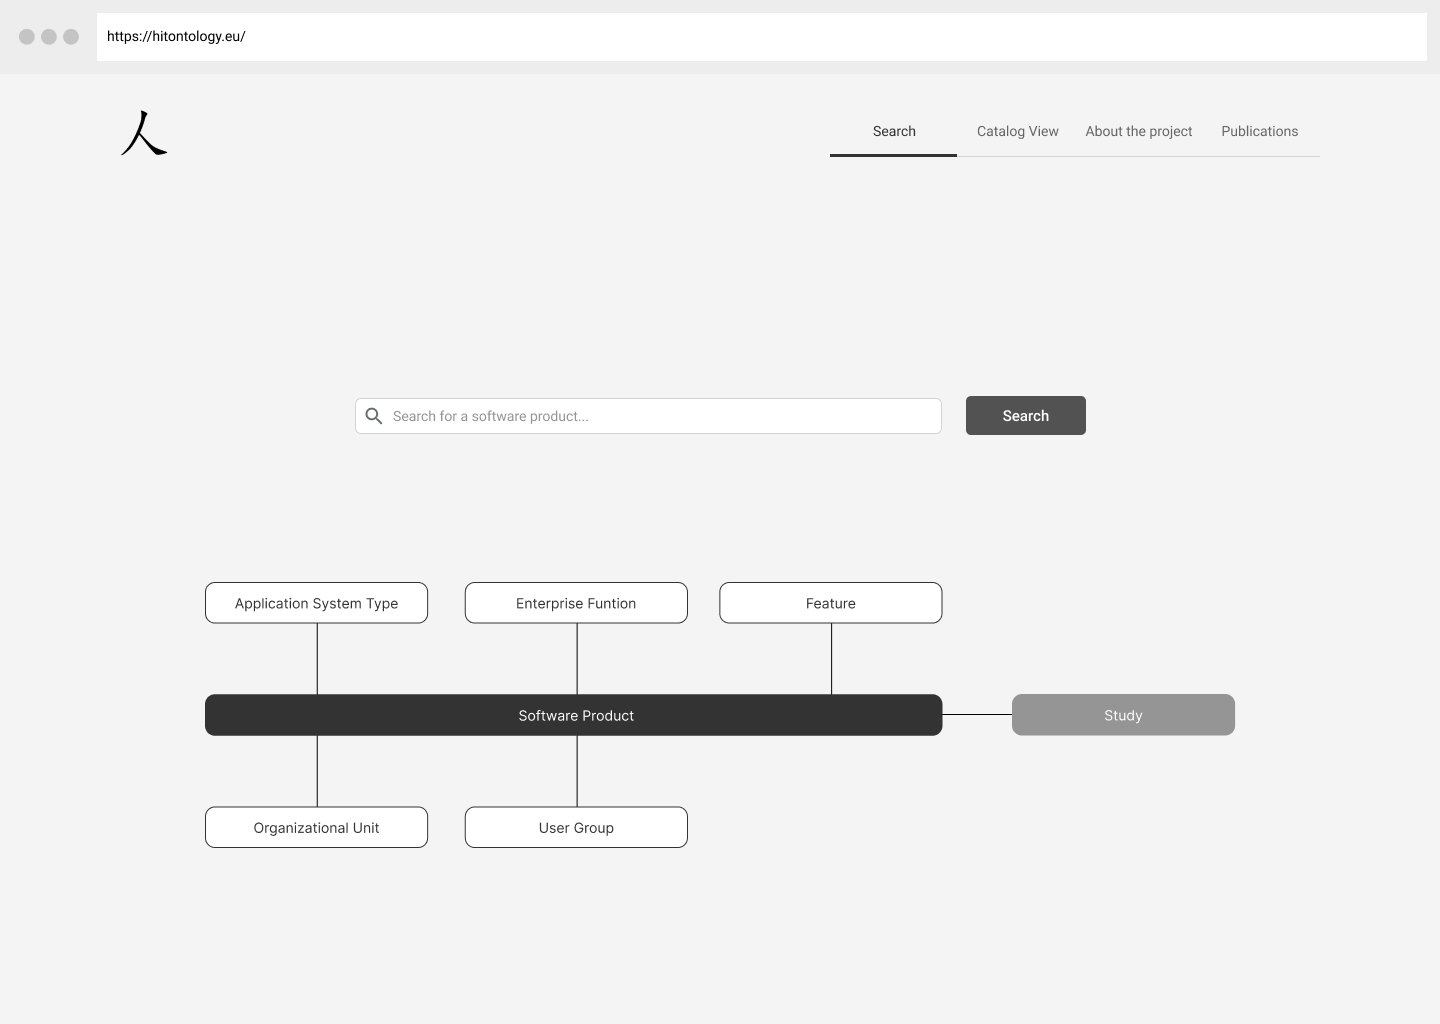
\includegraphics[width=1.45\textwidth, angle=-90]{Images/Startseite}
   	\caption{Lösung danach}
   	\label{fig:wireframe_start}
\end{figure}

\clearpage

\item \textbf{\enquote{Ästhetisches und minimalistisches Design}} \newline

In diesem Fall soll sichergestellt werden, dass das User Interface Design die Zielerreichung der Nutzer*innen unterstützt.



\begin{figure}[H]
	\centering
    	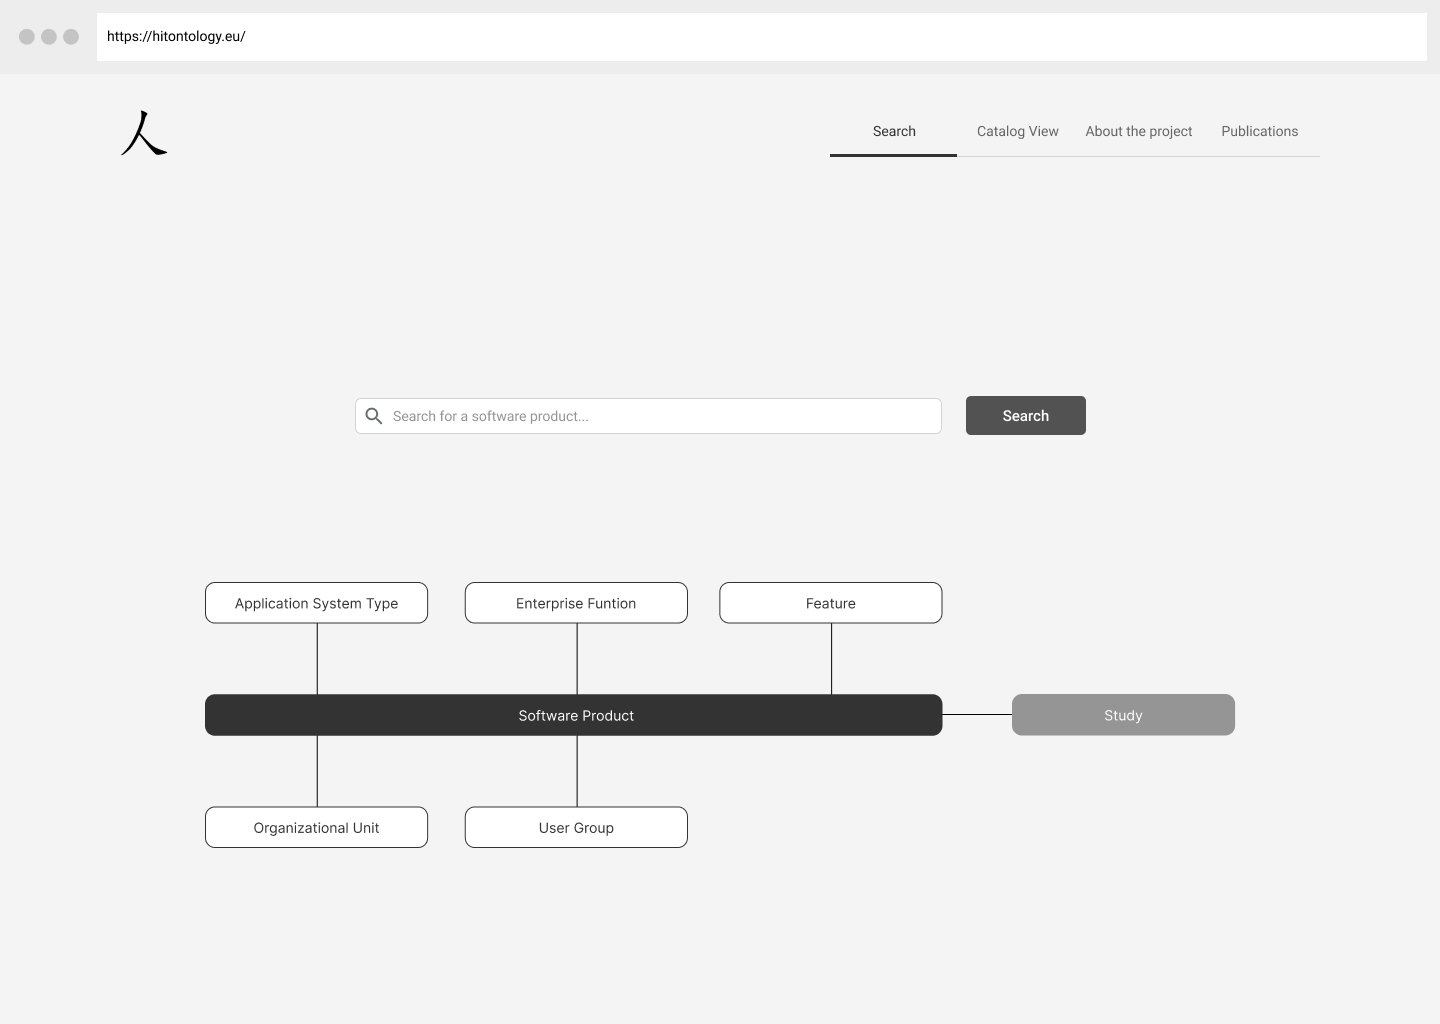
\includegraphics[width=1.45\textwidth, angle=-90]{Images/Startseite}
   	\caption{Lösung davor}
   	\label{fig:wireframe_start}
\end{figure}

\clearpage

\begin{figure}[H]
	\centering
    	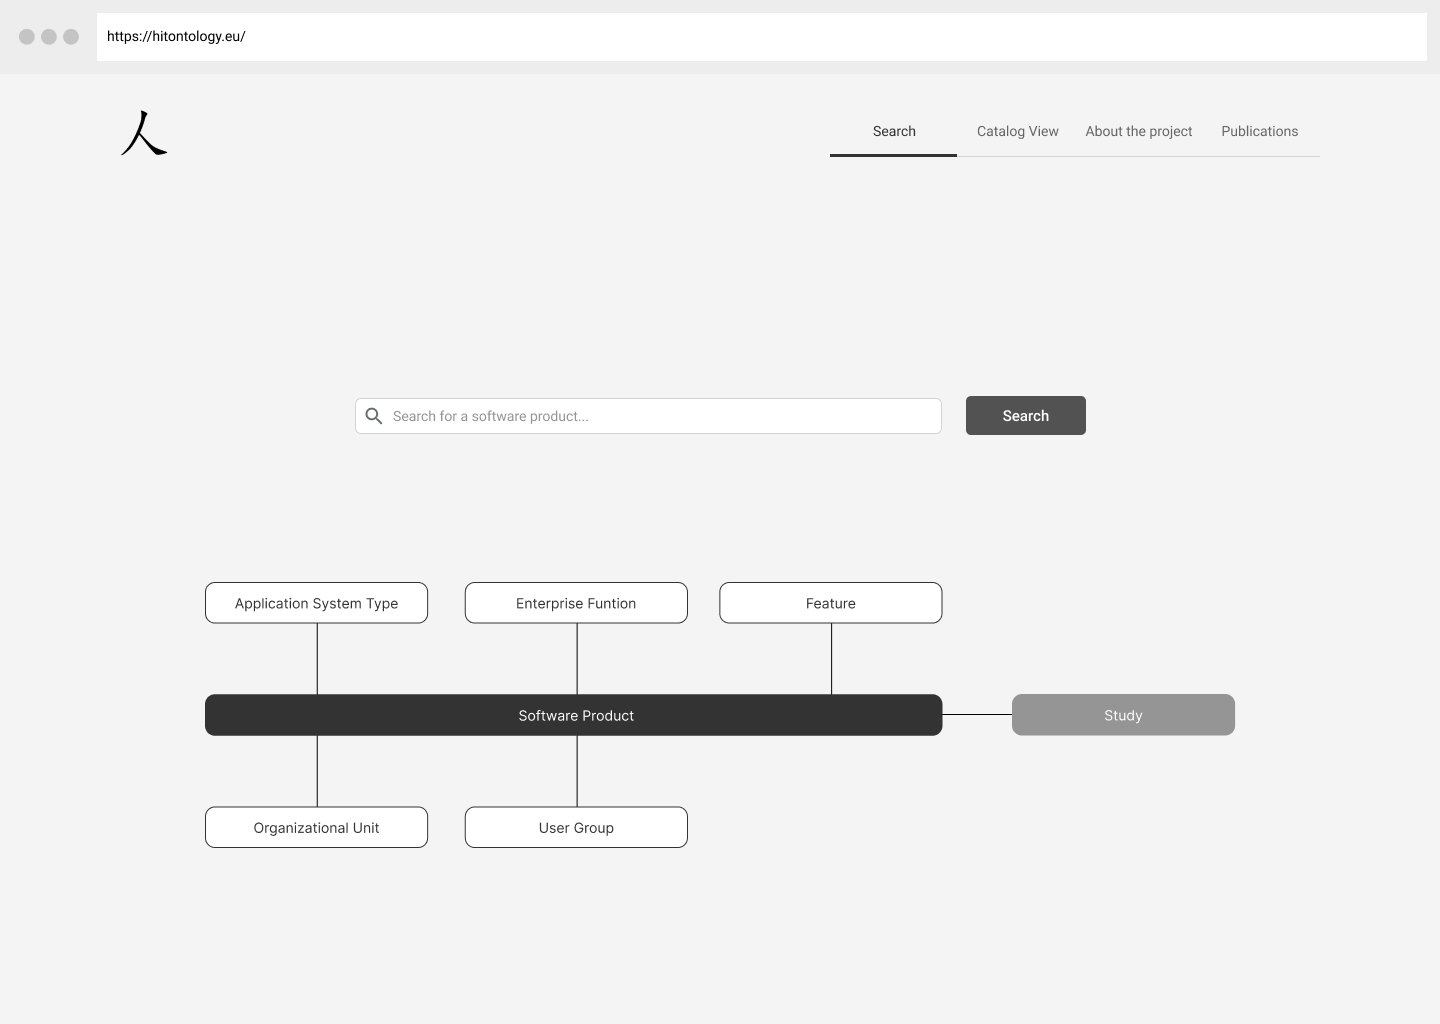
\includegraphics[width=1.45\textwidth, angle=-90]{Images/Startseite}
   	\caption{Lösung danach}
   	\label{fig:wireframe_start}
\end{figure}

\item \textbf{\enquote{Hilfe beim Erkennen, Diagnostizieren und Beheben von Fehlern}} \newline

Im Falle eines Fehlers soll Nutzer*innen klar gemacht werden, warum es zu diesem Fehler gekommen ist und wie dieses Fehler zu beheben ist.
Zum Beispiel liefert ein gesuchtes Begriff keine zutreffende Ergebnisse.
Demnach kann die Anwendung Nutzer*innen Feedback dazu geben und ihnen andere mögliche Suchbegriffe vorschlagen.
Siehe hier Abbildung \ref{point9_danach}
Aktuell bekommen Nutzer*innen keine Hilfestellung, wenn sie im Rahmen der facettierten Suche keine zutreffende Ergebnisse bekommen. 
Siehe hier Abbildung \ref{point9_davor}.

\begin{figure}[H]
	\centering
    	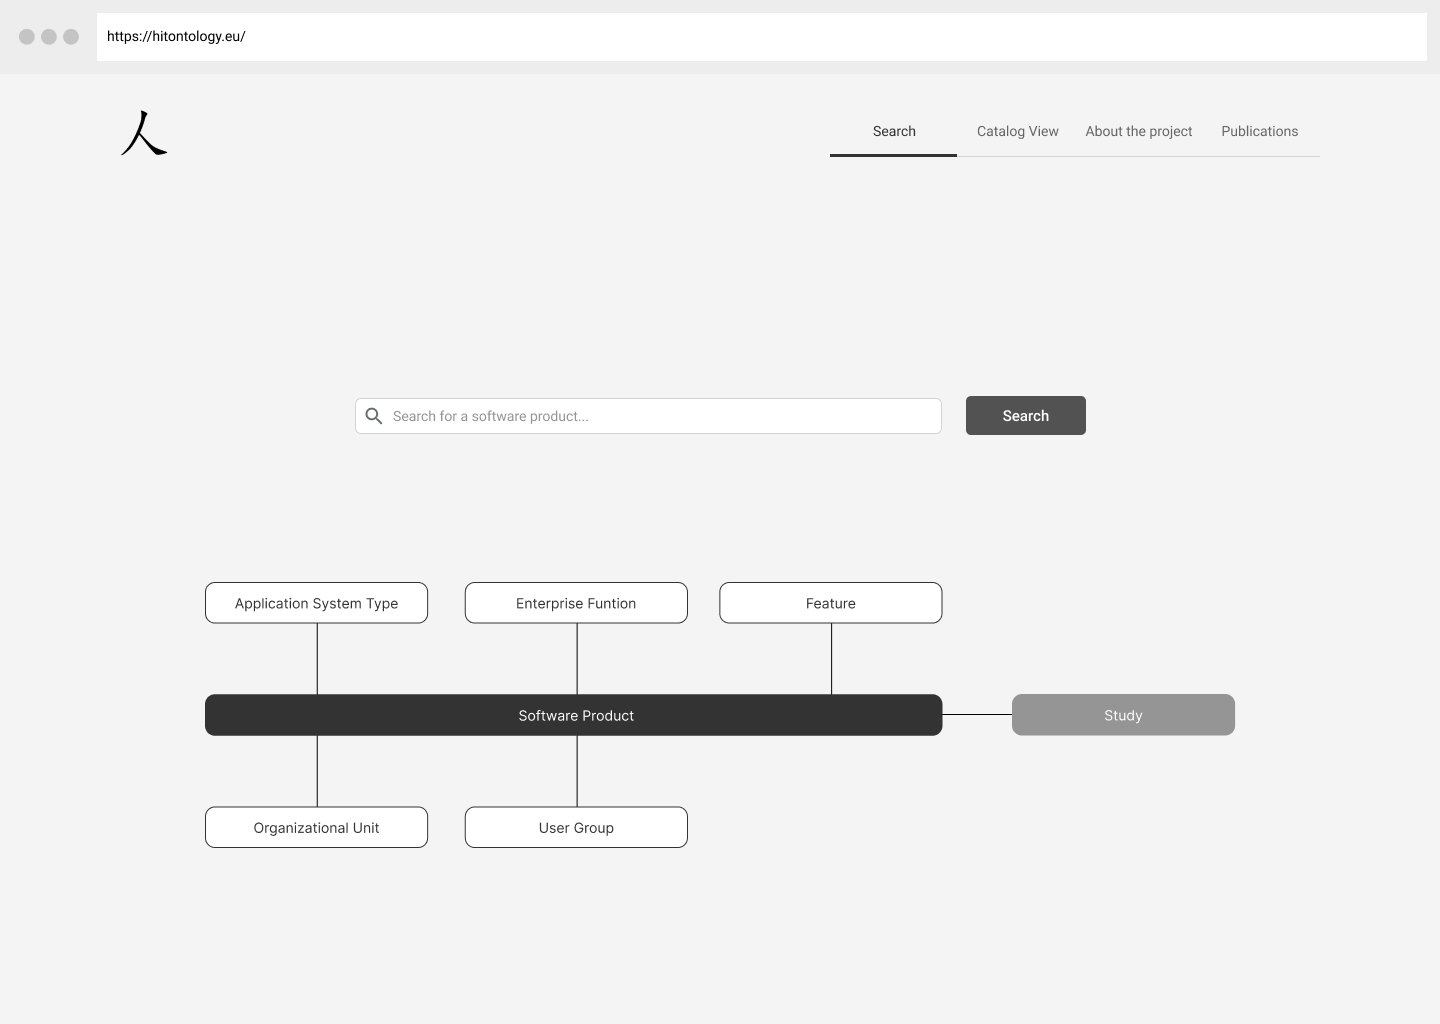
\includegraphics[width=1.45\textwidth, angle=-90]{Images/Startseite}
   	\caption{Lösung davor}
   	\label{fig:point9_davor}
\end{figure}

\begin{figure}[H]
	\centering
    	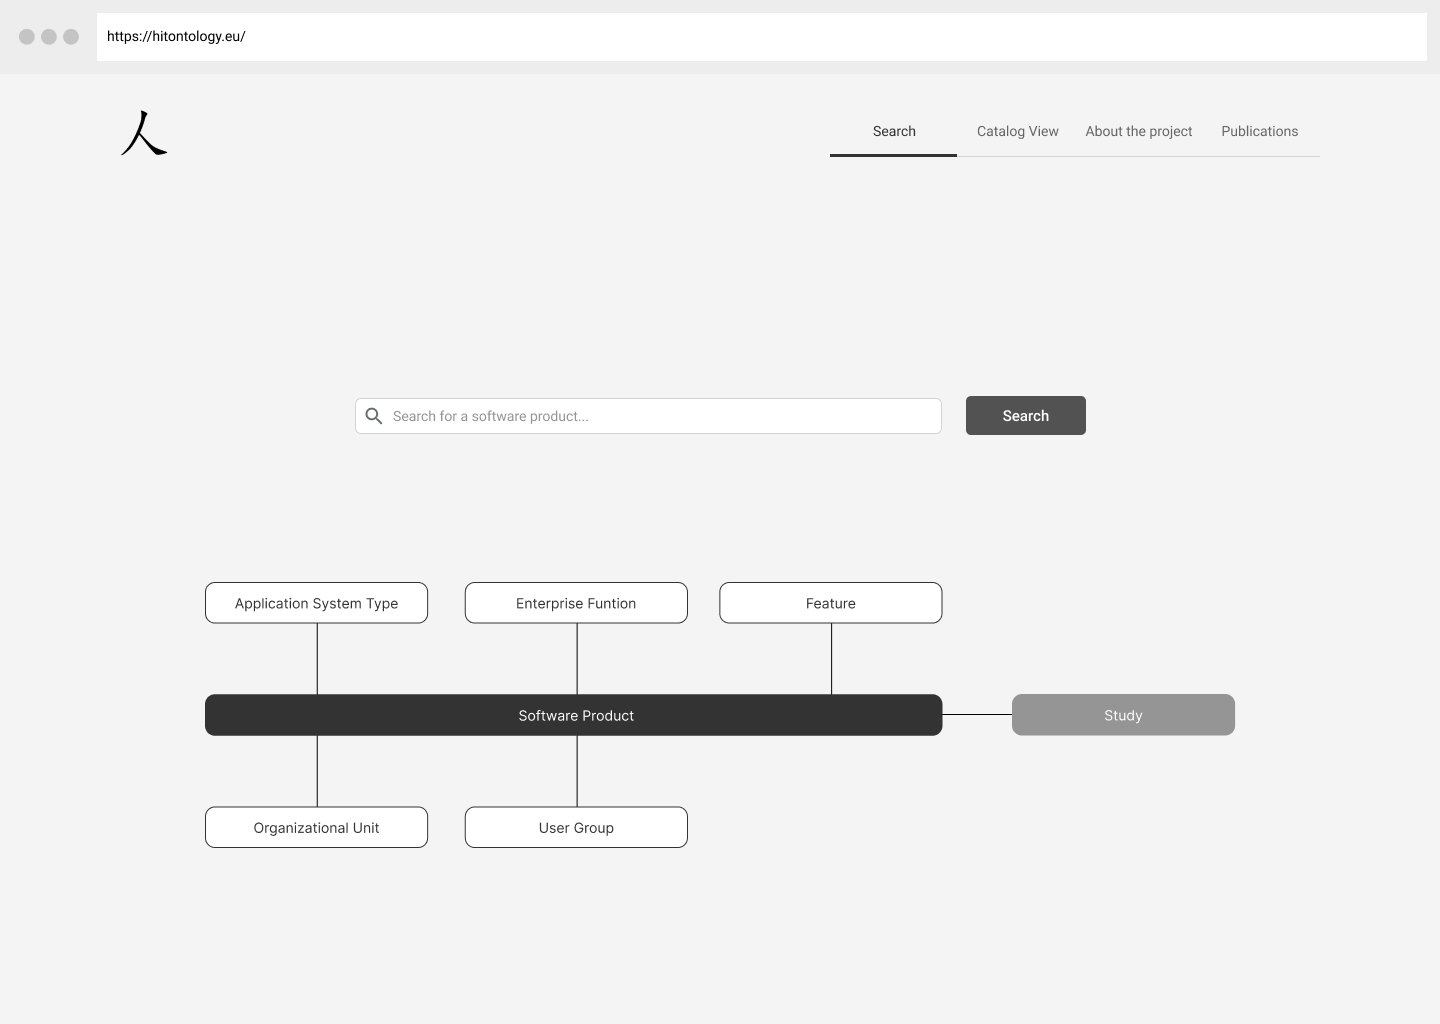
\includegraphics[width=1.45\textwidth, angle=-90]{Images/Startseite}
   	\caption{Lösung danach}
   	\label{fig:wireframe_start}
\end{figure}

\item \textbf{\enquote{Hilfe und Dokumentation}} \newline

Hilfe und Dokumentation sollten leicht auffindbar sein und auf die Aufgabe der Zielgruppen ausgerichtet sein. 


\begin{figure}[H]
	\centering
    	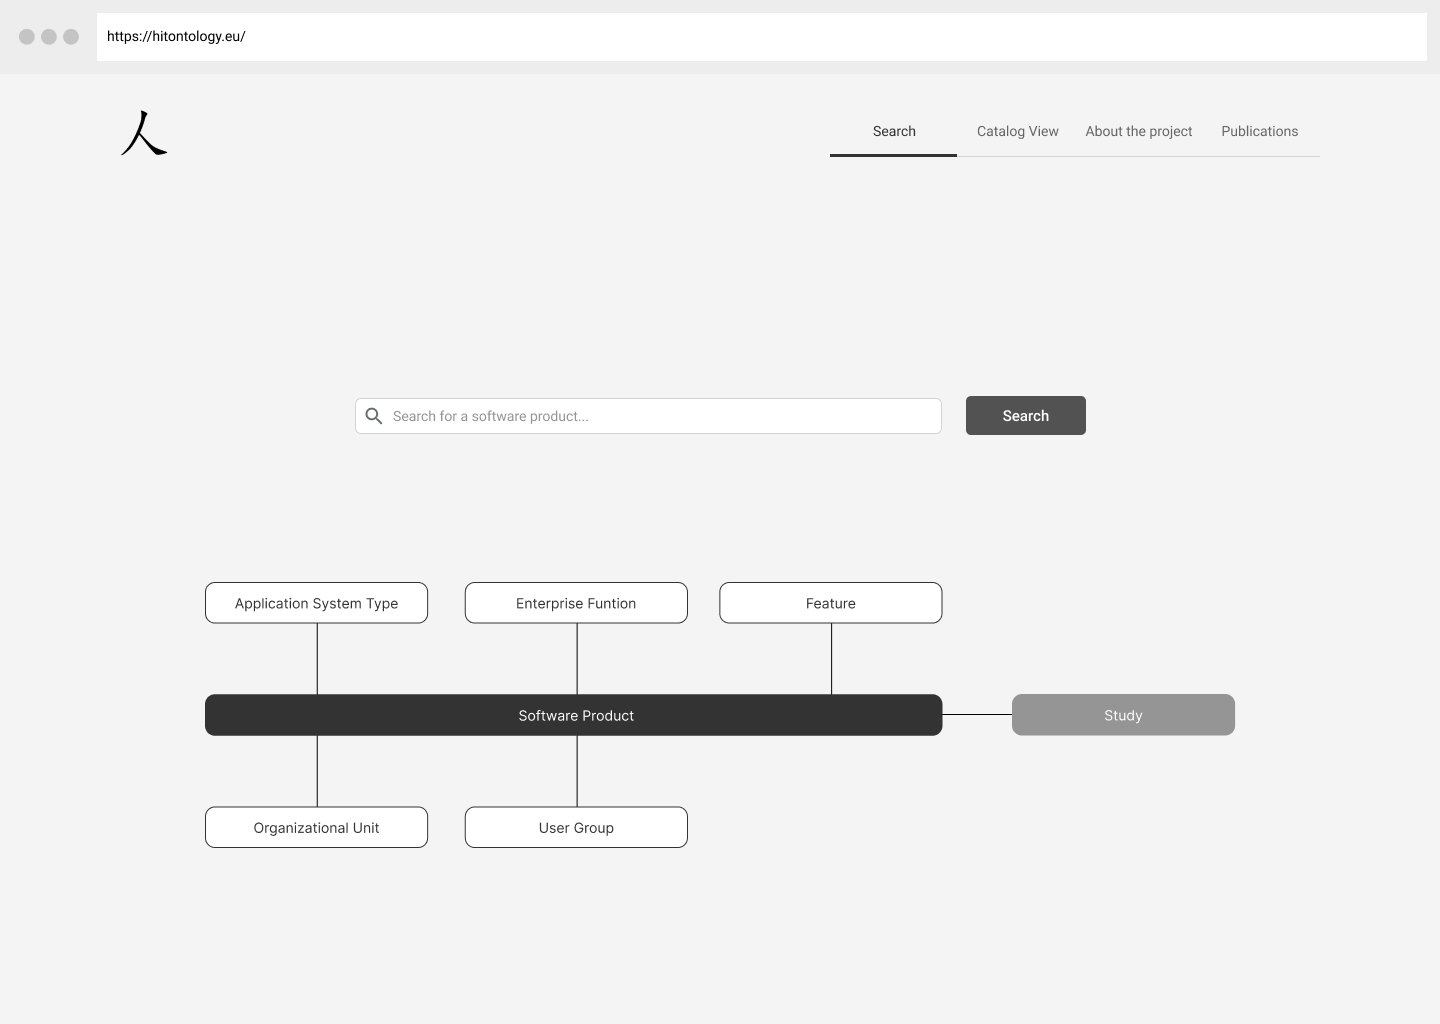
\includegraphics[width=1.45\textwidth, angle=-90]{Images/Startseite}
   	\caption{Lösung davor}
   	\label{fig:wireframe_start}
\end{figure}

\clearpage

\begin{figure}[H]
	\centering
    	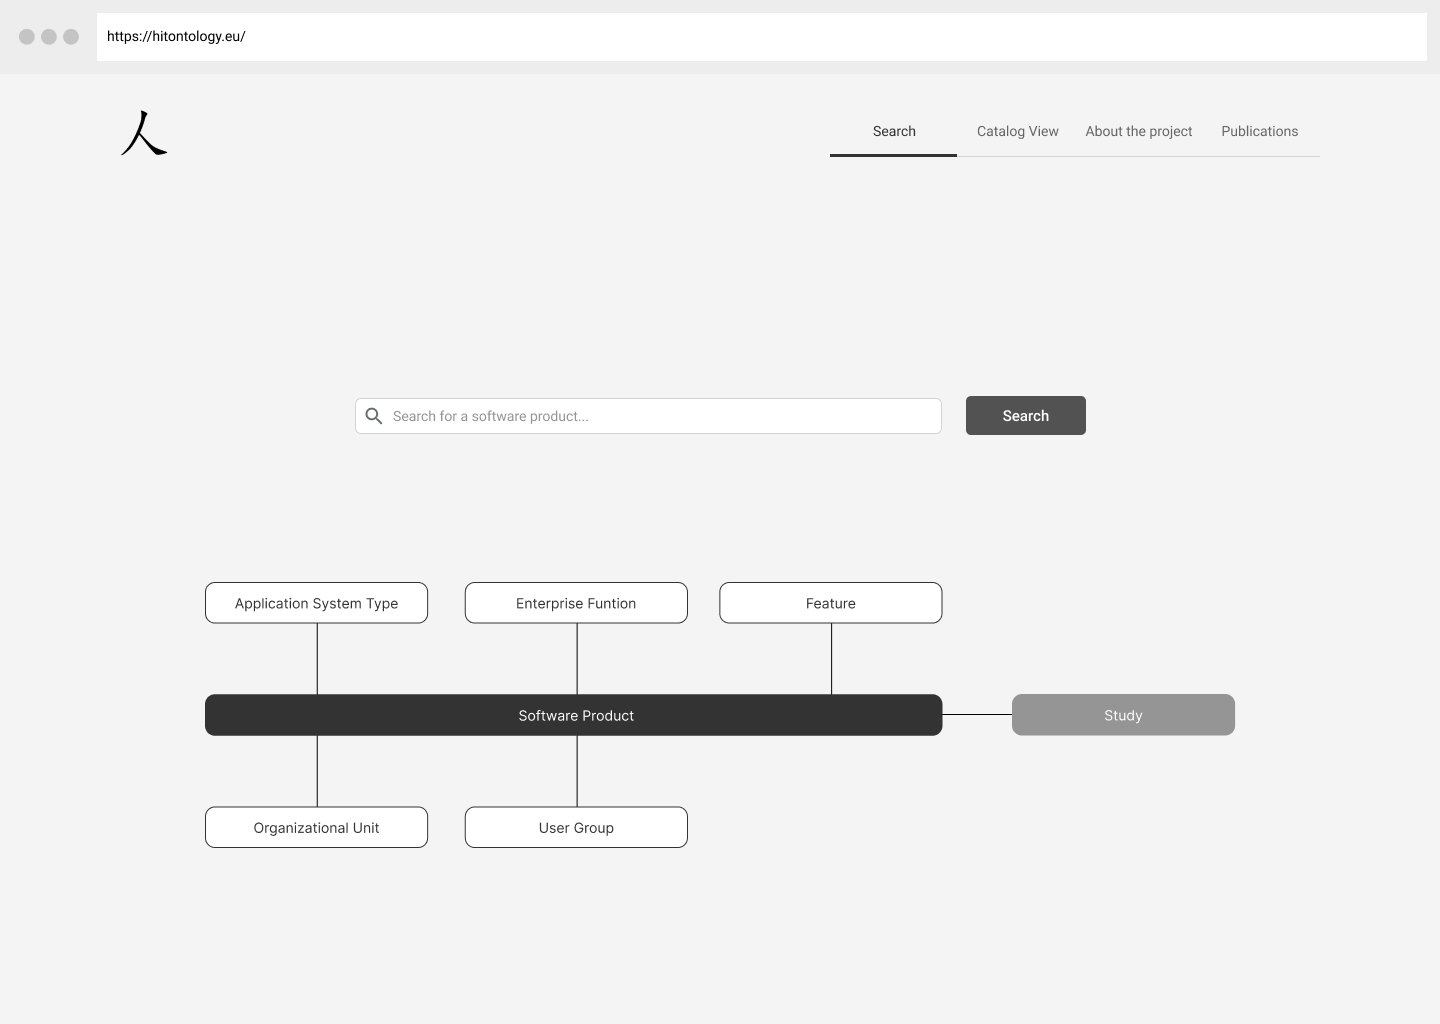
\includegraphics[width=1.45\textwidth, angle=-90]{Images/Startseite}
   	\caption{Lösung danach}
   	\label{fig:wireframe_start}
\end{figure}

\clearpage

\end{enumerate}
